\documentclass[10pt]{article}

% Preamble

\usepackage{amsmath,amsfonts,amssymb}
\usepackage[mathscr]{euscript}
%\usepackage[mathcal]{euscript}
\usepackage{mathrsfs}
\usepackage{graphicx}
\usepackage{float}
\usepackage{bbm}
\usepackage{braket}
\usepackage{tikz-feynman}
\usepackage{simpler-wick}
\usepackage{cancel}
\usepackage{stackengine}

\newcommand{\bigzero}{\mbox{\normalfont\Large\bfseries 0}}

\title{Notes On Advanced Quantum Field Theory \\ The Theory of Elementary Interactions \\ A Course Given By Dr. Tobias Osborne}
\author{Transcribed by Dr. Alexander V. St. John}

% The Document

\begin{document}

\maketitle

\clearpage

\section*{Lecture 1: Introduction}
\label{sec: lec1}

\noindent The goal for this course is to explain the current "standard model" for particle physics. This is too lofty of a goal for this course, so what we focus on is the textit{building blocks} of the standard model, such that we understand the origin and purpose of each term of the Lagrangian. \\

\noindent Topics covered include

\begin{enumerate}
\item Path integral quantization
	\subitem Via Gaussian integrals.
\item Review perturbation theory via path integrals
	\subitem Includes familiar tools for calculating correlation functions such as Wick's theorem, Feynman rules, etc.
\item Renormalization
	\subitem Allows us to discuss effective QFT (e.g., eliminating infinities) in more detail.
\item Abelian and nonabelian classical gauge theories
	\subitem Uses path integrals to deduce quantizations from classical field theories.
\item Quantization of non-abelian gauge theories
	\subitem Employs path integrals for perturbative calculations and lattices for nonperturbative calculations.
\item Spontaneous symmetry breaking mechanisms
\end{enumerate}

\subsection*{Path Integrals}

\noindent Let's first suppose that the quantization is already done, and we have a quantum system with a Hilbert space $\mathcal{H}$, a Hamiltonian $\hat{H}$, and a propagator from integrating the Schroedinger equation, $U(t) = e^{-i\hat{H}t}$. \\

\noindent Now work out a representation to first order for the propagator by Taylor expanding

\begin{equation}
U(t) = e^{-i\hat{H}t} = \left( e^{-\frac{it}{N}\hat{H}}  \right) ^N= \lim_{N \rightarrow \infty} \left( \mathbb{I} - \frac{it}{N}\hat{H} \right) ^N
\end{equation}

\noindent Let $\{ \ket{j} \}$ be a basis for the Hilbert space $\mathcal{H}$ and consider the transition amplitude of evolving from an eigenstate $\ket{\phi_i}$ to another eigenstate $\ket{\phi_f}$

\begin{equation}
\bra{\phi_f} U(t) \ket{\phi_i} = \bra{\phi_f}  \left( e^{-\frac{it}{N}\hat{H}}  \right) ^N \ket{\phi_i}
\end{equation}

\noindent Insert  $N-1$ Hilbert space basis completeness relations, one in between each of the $N$ exponentials, and note that the sum over all paths from initial state to final state of functions of the paths

\begin{align}
\bra{\phi_f} U(t) \ket{\phi_i} &= \sum_{j_1,\dots,j_{N-1}} \bra{\phi_f} e^{-\frac{it}{N}\hat{H}} \ket{j_{N-1}}\bra{j_{N-1}} e^{-\frac{it}{N}\hat{H}} \dots \ket{j_1}\bra{j_1} e^{-\frac{it}{N}\hat{H}} \ket{\phi_i} \\
&\equiv \sum_{\text{paths}} f(j_1, \dots , j_{N-1}).
\end{align}

\noindent So, the transition amplitude of this state evolution is a sum over all of the paths through the basis states $j_1,\dots,j_{N-1}$. An example schematic of a path is visualized below.

\begin{figure}[H]
	\centering
	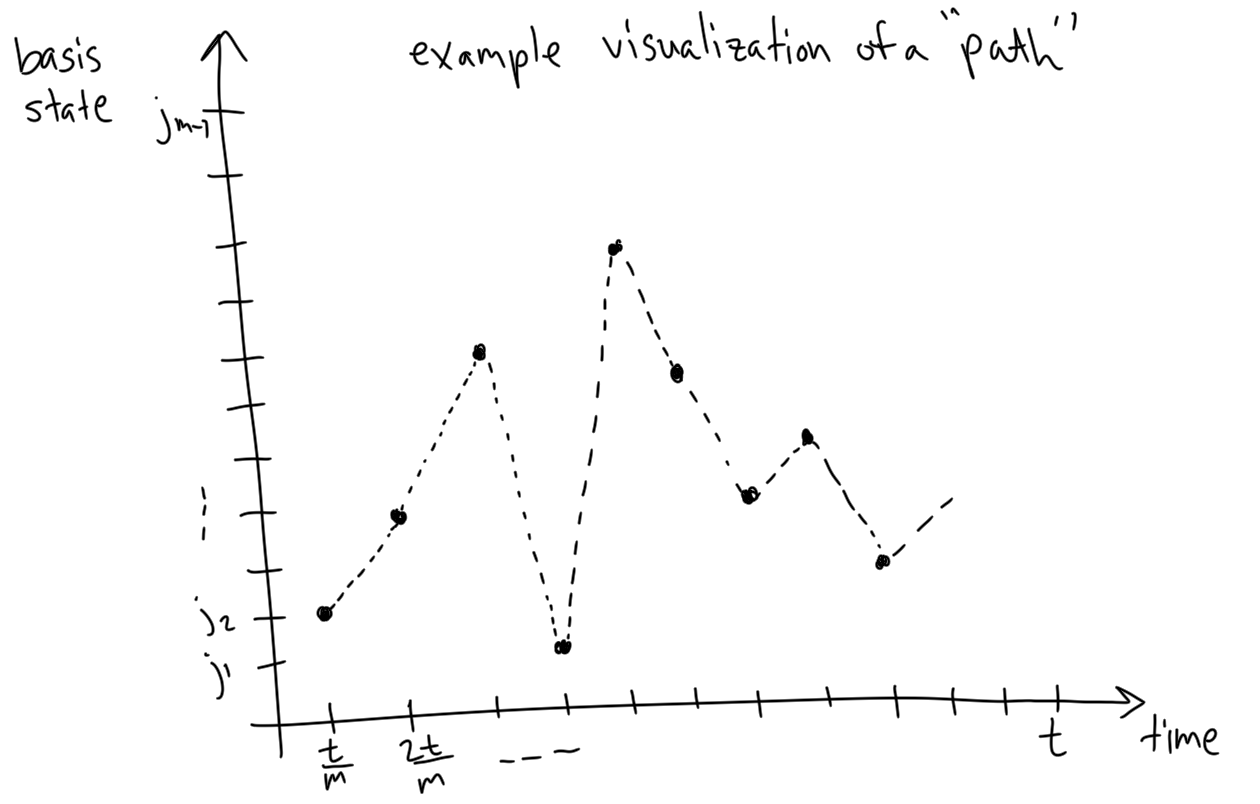
\includegraphics[width=4in]{images/pathviz.png}
	\caption*{}
\end{figure}

\noindent To work out the function of the path $f(j_1, \dots, j_{N-1})$, we need to calculate these individual transition amplitudes between successive states $\ket{j_{k-1}}$ to some final state $\bra{j_k}$ in the path integral setting, and seek to write it as an exponential of some function of the states $\mathcal{L}(j_{k-1}, j_k)$, the Lagrangian density

\begin{equation}
\bra{j_k} (\mathbb{I} - \frac{it}{N} \hat{H}) \ket{j_{k-1}} \simeq e^{\frac{it}{N} \mathcal{L}(j_{k-1}, j_k)}.
\end{equation}

\noindent So, the full transition amplitude will be a product of exponentials pf Lagrangian densities, well-known classical quantities

\begin{equation}
\bra{\phi_f} U(t) \ket{\phi_i} = \sum_{\text{paths}} f(j_1, \dots , j_{N-1}) = \sum_{j_1,\dots,j_{N-1}} e^{\frac{it}{N} \sum_{k=2}^{N-1} \mathcal{L} (j_{k-1}, j_k) } .
\end{equation}

\noindent Before moving forward, what makes the path integral so interesting?

\begin{enumerate}
\item It allows the calculation of quantum quantities, the transition amplitudes, via well-understood classical solutions and methods for handling highly oscillatory integrals such as the saddle point method.
\item It can also be used to build nonperturbative approximation schemes, such as Monte Carlo sampling over paths.
\end{enumerate}

\subsection*{Example: General Nonrelativistic Quantum Mechanical System}

\noindent Let's assume a little bit more about our quantum system. Suppose the quantum system is inspired by a classical system with pairs of canonical coordinates and momenta and the Hamiltonian $H(\{q^j\},\{p^j\}) = H(q,p)$. \\

\noindent Turn around the path integral sum over paths to guess a quantum Hamiltonian and Hilbert space from this classical Hamiltonian via

\begin{equation}
U(q_i, q_f, T) = \bra{q_f} U(T) \ket{q_i} = \bra{q_f} e^{-iT\hat{H}} \ket{q_i}
\end{equation}

\noindent Proceed as before, mulitplying the exponentials and inserting $N-1$ completeness relations in between the $N$ copies of the exponential. The completeness relation for the canonical position basis, a continuous variable, is

\begin{equation}
\mathbb{I} = \left( \prod_j \int dq_k^j \right) \ket{q_k} \bra{q_k}
\end{equation}

\noindent So, the transition amplitude in this case is, with $\epsilon \equiv \delta t = \frac{T}{N}$

\begin{equation}
\bra{q_f} U(T) \ket{q_i} = \sum_{k_1,\dots,k_{N-1}} \bra{q_f} e^{-i \epsilon \hat{H}} \ket{q_{k_{N-1}}} \bra{q_{k_{N-1}}} \dots \ket{q_{k_1}}\bra{q_{k_1}} e^{-i \epsilon \hat{H}} \ket{q_i}.
\end{equation}

\noindent There are three cases for the dependence of the quantum Hamiltonian on the canonical coordinates in the expression for the propagator. It can depend purely on position, purely on momenta, or most realistically, it can depend on both. \\

\noindent In the case that the Hamiltonian is a function purely dependent on canonical position, such that $\hat{H} = g(\hat{q})$, we easily calculate the transition amplitude, which relates the quantum and classical canonical positions, since the $\ket{q_k}$ are energy eigenstates of the position-dependent Hamiltonian

\begin{align}
\bra{q_{k+1}} g(\hat{q}) \ket{q_k} &= g(q_k) \prod_j \delta ( q_k^j - q_{k+1}^j ) \\
&= g \left( \frac{q_{k+1} + q_k}{2} \right) \left( \prod_j \int \frac{dp_k^j}{2\pi} \right) e^{ i \sum_j p_k^j (q_{k+1}^j - q_k^j ) }.
\end{align}

\noindent Where we used the Dirac delta distribution identity $\delta (q) = \int_{-\infty}^{\infty} \frac{dp}{2\pi} \, e^{i p \cdot q}$ to introduce the canonical momenta into the transition amplitude. Also note that the Dirac delta function forces $q_{k+1} = q_k$, such that $f(q_k) = f(\frac{q_{k+1} + q_k}{2})$, and we write it in this fashion for later use. \\

\noindent Next, in the case that the Hamiltonian is a function purely dependent on canonical momenta, such that $\hat{H} = h(\hat{p})$, the transition amplitude is calculated by inserting the completeness relation for the momentum eigenbasis.

\begin{align}
\bra{q_{k+1}} h(\hat{p}) \ket{q_k} &= \bra{q_{k+1}} h(\hat{p}) \cdot \prod_j \int dp_k^j \ket{p_k} \braket{p_k | q_k} \\
&= \prod_j \int \frac{dp_k^j}{2\pi} \, h(p_k) e^{ i \sum_j p_k^j (q_{k+1}^j - q_k^j ) }
\end{align}

\noindent Where the inner product of the position and momentum eigenstates is a Fourier phase element $\braket{p | q} = \frac{1}{2\pi} e^{i p \cdot q}$, and we get the sum, since the subscript $k$ denotes $N$ total canonical coordinate pairs. \\

\noindent The more realistic situation is when the Hamiltonian is dependent on both position and momenta $\hat{H} = \hat{H}(\hat{q}, \hat{p}) = g(\hat{q}) + h(\hat{p})$. Suppose the dependencies are linearly separable in the quantum Hamiltonian. Then we may translate between classical position and momenta via the Taylor expansion to first order

\begin{equation}
e^{-i \epsilon \hat{H}} = \mathbb{I} - i \epsilon \hat{H} = \mathbb{I} - i \epsilon (g(\hat{q}) + h(\hat{p})).
\end{equation}

\noindent Using this linearity, we can write this dependence in the derived formula as

\begin{equation}
\bra{q_{k+1}} e^{-i \epsilon \hat{H}(\hat{q}, \hat{p})} \ket{q_k} = \prod_j \int \frac{dp_k^j}{2\pi} \, e^{ -i \epsilon H (\frac{q_{k+1}+q_k}{2}, p_k)} e^{ i \sum_j p_k^j (q_{k+1}^j - q_k^j ) }
\end{equation}

\noindent Putting all this together into the propagator, which is really the transition amplitude for a nonrelativistic quantum system,

\begin{equation}
U(q_i, q_f; T) = \left(  \prod_{jk} \int dq_k^j \int \frac{p_k^j}{2\pi} \right) e^{i \sum_k \left( \sum_j p_k^j (q_{k+1}^j - q_k^j) - \epsilon H (\frac{q_{k+1} + q_k}{2}, p_k) \right)}.
\end{equation}

\noindent Take note that there is nothing quantum on the RHS: no hats! We have used purely classical data to define the quantum propagator, or, transition amplitude, on the LHS, such that $U(q_i, q_f; T) \propto e^{- i \epsilon H (q_i, q_f; T)}$. \\

\noindent A few other remarkable points:

\noindent Using the saddle point method, we can build an approximation scheme for $U$. This is useful for solving highly oscillatory integrals, as we see in the transition amplitude above (e.g., $e^{i\dots}$), since such integrals can be approximated by its saddle points (or critical points), which correspond to classical paths of the system. \\

\noindent Monte Carlo sampling of the system can also be used to approximate the transition amplitude by building an estimator for the RHS, sampling over classical configurations, and summing up the estimator. \\

\noindent Now, the expression for $U$ was not-so-pretty, but imagine continuous time variables and integrals when you see $\sum_k$ and $\epsilon$ above. In the limit as $N \rightarrow \infty$ (the number of completeness relations inserted), the quantum propagator is expressed in a continuous form with strange new "integrals".

\begin{equation}
U(q_i, q_f; T) = \left( \int \mathcal{D}q \int \mathcal{D} p \right) e^{i \int_0^T dt \, (\sum_j p^j \dot{q}^j - H(q,p))}
\end{equation}

\noindent Do not think of these as literal integrals, as we do not have a proper measure space to integrate over. Think of them as algorithms for now, something totally new that will be applied to solve this expression above.

\clearpage

\section*{Lecture 2: Gaussian Path Integrals}
\label{sec: lec2}

\noindent Recall the propagator, or transition amplitude, for a nonrelativistic quantum system

\begin{equation}
U(q_i, q_f; T) = \left( \prod_j \int \mathcal{D} q^j (t) \int \mathcal{D} p^j (t) \right) e^{i \int^T_0 dt \, \mathcal{L} (q^j, \dot{q}^j)}.
\end{equation}

\noindent To work with this, we often discretize $q(t) \rightarrow q^j_k$

\begin{figure}[H]
	\centering
	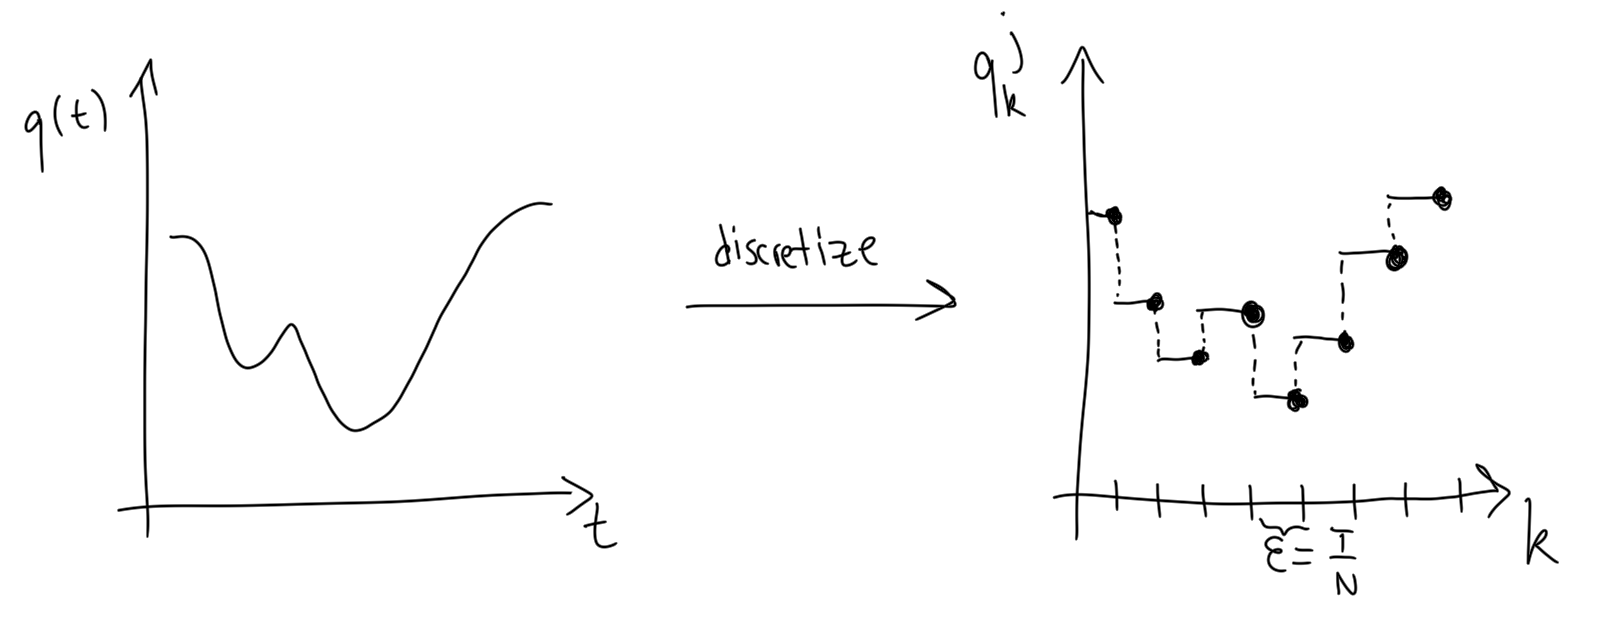
\includegraphics[width=4in]{images/discretize.png}
\end{figure}

\begin{equation}
U(q_i, q_f; T) = \left( \prod_{j, k} \int dq^j_k \int \frac{dp^j_k}{2\pi} \right) e^{i \sum_k (\sum_j p_k^j (q_{k+1}^j - q_k^j ) - \epsilon H)}
\end{equation}

\noindent Evaluate these very many integrals to get an answer dependent on $\epsilon = \frac{T}{N}$, since we discretized, take the limit as $\epsilon \rightarrow 0$ and deal with any encountered infinities.

\subsection*{Key Example}

\noindent Consider the classical Hamiltonian

\begin{equation}
H = \frac{p^2}{2 m} + V(q).
\end{equation}

\noindent Calculate the transition amplitude (\textbf{Exercise})

\begin{align}
U(q_i, q_f; T) &= \left( \prod_{j, k} \int dq^j_k \int \frac{dp^j_k}{2\pi} \right) e^{i \sum_k (\sum_j p_k^j (q_{k+1}^j - q_k^j ) - \epsilon H)} \\
&=  \left( \prod_{k} \int dq_k \int \frac{dp_k}{2\pi} \right) e^{i \sum_k (p_k (q_{k+1} - q_k ) - \epsilon (\frac{p_k^2}{2m} + V(q)) )} \\
&= \left( \prod_k \int dq_k \right) \sqrt{\frac{-im}{2\pi \epsilon}} e^{i \sum_k \frac{m}{2\epsilon} (q_{k+1} - q_k)^2 - \epsilon V(\frac{q_{k+1} + q_k}{2})}.
\end{align}

\noindent We may also write this in the following notation, using the fact that the argument of the exponential is the discretized version of the action, now without the $p$-integral

\begin{equation}
\lim_{\epsilon \rightarrow 0} U(q_i, q_f; T) = \int \mathcal{D} q(t) e^{\mathcal{S}[q(t)]}
\end{equation}

\noindent Where the action is 

\begin{equation}
\mathcal{S}[q(t)] = \int^T_0 dt \,\, (\frac{m}{2} \sum_j (\dot{q}^j)^2 - V(q)).
\end{equation}

\noindent Note that if our system is a harmonic oscillator $V(q) = \frac{1}{2} m \omega q^2$, we can do the full integral.

\subsection*{Path Integrals for Scalar Fields}

\noindent Recall the classical scalar field with Lagrangian density and Hamiltonian

\begin{align}
\mathcal{L} &= \frac{1}{2} (\partial_\mu \phi)^2 - V(\phi) \\
H &= \int d^3 x \,\, (\frac{1}{2} \pi^2 + \frac{1}{2} (\nabla \phi)^2 + V(\phi) ).
\end{align}

\noindent The path integral prescription for quantum scalar fields gives the transition amplitude, by blind application of the above, we conjecture that

\begin{equation}
\bra{\phi_b} e^{-i \hat{H} T} \ket{\phi_a} = \left( \int \mathcal{D} \phi \int \mathcal{D} \pi \right) e^{i \int^T_0 d^4x \, (\pi \dot{\phi} - H(\phi)}
\end{equation}

\noindent Where the boundary terms are $\phi(t=0, x) = \phi_a (x)$ and $\phi(t=T, x) = \phi_b (x)$. \\

\noindent As explained above, to make sense of this quantity, we must discretize, evaluate, and take the continuum limit as $\epsilon \rightarrow \infty$. When we discretize, note that we only discretize space, as discretizing time in this way will cause trouble with the conjugate momenta. \\

\noindent The field operators are discretized over a "grid" of points $x_j$ each of width $\epsilon$, such that

\begin{equation}
\phi(t, x) \,\,\, \rightarrow \,\,\, \phi(t, x_j) \equiv q^j (t).
\end{equation}

\noindent Then discretize the integral by turning it into a sum over the grid

\begin{equation}
\int d^3 x  \,\,\, \rightarrow \,\,\, \epsilon^3 \Sigma_{j \in \mathbb{Z}^3} .
\end{equation}

\noindent Next the derivative can be discretized via a finite difference. Note that much better choices of a symmetric difference can be used, which are more computationally nice.

\begin{equation}
\nabla_\mu \phi(x) \,\,\, \rightarrow  \,\,\, \frac{(\phi(x_j + \epsilon_\mu) - \phi(x_j))}{|\epsilon_\mu|}.
\end{equation}

\noindent Where $\mu$ chooses one of four directions to calculate the derivative, and

\begin{equation}
\epsilon_{\mu} = \epsilon \{ \left(\begin{smallmatrix}1\\0\\0\\0\end{smallmatrix}\right), \left(\begin{smallmatrix}0\\1\\0\\0\end{smallmatrix}\right), \left(\begin{smallmatrix}0\\0\\1\\0\end{smallmatrix}\right), \left(\begin{smallmatrix}0\\0\\0\\1\end{smallmatrix}\right) \}
\end{equation}

\noindent And, lastly, the potential just becomes evaluated at each $x_j$

\begin{equation}
V(\phi(x)) \,\,\, \rightarrow \,\,\, V(\phi(x_j)).
\end{equation}

\noindent Then the Lagrangian is discretized to a sum over a bunch of terms (\textbf{Exercise}), but the only relevant term to the construction of the Hamiltonian is the time derivative of the field operator $\dot{\phi}$

\begin{equation}
L = \int d^3 x \, \mathcal{L} \rightarrow \epsilon^3 \sum_j \frac{1}{2} (\dot{\phi}_j)^2
\end{equation}

\noindent And the discretized conjugate momentum becomes

\begin{equation}
\pi^j = \frac{\partial L}{\partial \dot{q}^j} = \frac{\partial L}{\partial \dot{\phi}^j}  \,\,\, \rightarrow \,\,\, \epsilon^3 \dot{q}^j
\end{equation}

\noindent Finally, we have the discretized Hamiltonian, where we display the $\epsilon$ terms to show that if we did not add the $\epsilon^3$ term to the discretized Lagrangian, we would be stuck with an extra $\epsilon^{-3}$ on the discretized Hamiltonian

\begin{equation}
H = \epsilon^3 \sum_j \epsilon^{-3} \pi_j^2 + \frac{1}{2} \left( \frac{q_{j+\epsilon^\mu}-q_j}{\epsilon} \right)^2 + V(q).
\end{equation}

\noindent In summary, the discretization of the scalar field gives us a nonrelativistic lattice system such that the discretized Hamiltonian is the sum of a kinetic energy term and a potential energy term. The second step is to evaluate the (nonrelativistic) path integral, and the third step is to take the continuum limit as $\epsilon \rightarrow 0$, which will later be re-branded as renormalization. \\

\noindent The most important case of the scalar field is the quadratic potential, which corresponds to the Klein-Gordon field (e.g., discretizing Klein-Gordon theory yields the quadratic potential below), is

\begin{equation}
V(q) = \frac{1}{2} q^T \textbf{A} q.
\end{equation}

\subsection*{Gaussian Integrals}

\noindent Consider the following integral 

\begin{equation}
I = \int_{-\infty}^\infty dx \,\, e^{-x^2} = \sqrt{\pi}.
\end{equation}

\noindent Proof:

\begin{align}
I &= \int_{-\infty}^\infty dx \,\, e^{-x^2} \\
I^2 &= \left(\int_{-\infty}^\infty dx \,\, e^{-x^2} \right) \left( \int_{-\infty}^\infty dy \,\, e^{-y^2}  \right) \\
&= \int_0^\infty r dr \, \int_0^{2\pi} d\theta \, e^{-r^2} \\
I^2 &= 2 \pi \int_0^\infty \frac{d}{dr} \left( -\frac{1}{2} e^{-r^2} \right) dr = \pi
\end{align}

\noindent This is actually a special case of the more general form

\begin{align}
\int_{-\infty}^\infty dx \,\, e^{ -\frac{1}{2} a x^2 + b x } &= \sqrt{\frac{2\pi}{a}} e^{ \frac{b^2}{2a}  } \\
\int_{-\infty}^\infty dx \,\, e^{  i a x^2 + i b x } &= \sqrt{\frac{2\pi i}{a}} e^{ \frac{-i b^2}{2a}  } \\
\end{align}

\noindent We will extensively use the moments generated by the Gaussian integrand

\begin{align}
\langle x^n \rangle = \frac{\int_{-\infty}^\infty dx \,\, x^n e^{ -\frac{1}{2} a x^2}}{\int_{-\infty}^\infty dx \,\, e^{ -\frac{1}{2} a x^2}}.
\end{align}

\noindent Note that if $n$ is odd, then the moment is zero. So, rewrite the exponent as $2m$. Then (\textbf{Exercise})

\begin{equation}
\langle x^{2m} \rangle = \frac{(2m-1)!!}{a^m}.
\end{equation}

\noindent Note that the double factorial $(2m-1)!!$ represents the number of ways to join $2m$ points in pairs. -- "All science should in linear algebra or combinatorics." -- \\

\noindent Another closed form of this integral is in terms of derivatives

\begin{align}
\langle x^{2m} \rangle &=  \left( \frac{d}{db} \right)^{2m} \left(  \frac{\int_{-\infty}^\infty dx \,\, e^{ -\frac{1}{2} a x^2 + b x }}{\int_{-\infty}^\infty dx \,\, e^{ -\frac{1}{2} a x^2 }} \right) \big|_{b=0} \\
&= \left( \frac{d}{db} \right)^{2m} e^{\frac{b^2}{2a}} \big|_{b=0}.
\end{align}

\noindent To evaluate Gaussian integrals of many variables, where $x \in \mathbb{R}^n$, consider

\begin{equation}
I(\textbf{A}, B) = \int_{-\infty}^\infty dx_1 \dots \int_{-\infty}^\infty dx_n \,\, e^{-x^T \textbf{A} x + B^T x}
\end{equation}

\noindent Where $\textbf{A}$ is an $n \times n$ symmetric real matrix and $B$ is an $n \times 1$ real vector. Since $\textbf{A}$ is real, symmetric, it contains orthogonal $\textbf{O}$ and diagonal matrices $\textbf{D}$, such that $\textbf{O}^T \textbf{O} = \mathbb{I}$ and $\textbf{D}$ is diagonalized with the eignevalues of $\textbf{A}$.

\begin{equation}
\textbf{O}^T \textbf{D} \textbf{O} = \textbf{A}
\end{equation}

\noindent Assume that $B=0$ and define $y = \textbf{O} x$. Then

\begin{align}
I(\textbf{A}, B=0) &= \int_{-\infty}^\infty dy_1 \dots \int_{-\infty}^\infty dy_n \,\, e^{-y^T \textbf{D} y} \\
&= \prod_{j=1}^n \int_{-\infty}^\infty dy_j \,\, e^{-y_j^2 \lambda_j} \\
&= \prod_{j=1}^n \sqrt{\frac{\pi}{\lambda_j}} \\
I(\textbf{A}, B=0)&= \sqrt{\frac{\pi^n}{det(\textbf{A})}}.
\end{align}

\noindent The $B \ne 0$ case (\textbf{Exercise}) results in the following

\begin{equation}
I(\textbf{A},B) = \sqrt{\frac{\pi^n}{det(\textbf{A})}} e^{B^T \textbf{A}^{-1} B}.
\end{equation}

\clearpage

\section*{Lecture 3: Correlation Functions and Path Integrals}
\label{sec: lec3}


\noindent Recall the generating function for a single-variable Gaussian probability distribution $e^{\frac{1}{2} a x^2}$ and the moment-generating integral

\begin{equation}
I = \int_{-\infty}^\infty dx \,\, x^{2n} e^{\frac{1}{2} a x^2} = \frac{(2n-1)!!}{a^n}.
\end{equation}

\noindent We also derived the identity with the generating function for the multivariable Gaussian probability distribution

\begin{equation}
\int_{-\infty}^\infty dx_1 \dots \int_{-\infty}^\infty dx_n \,\, e^{-\frac{1}{2} x^T \textbf{A} x + J^T x} = \sqrt{\frac{\pi^n}{det(\textbf{A})}} e^{J^T \textbf{A}^{-1} J}.
\end{equation}

\noindent The 2-point correlation function for the $n$-variable Gaussian is (\textbf{Exercise}), for $j \ne k$

\begin{equation}
\langle x_j x_k \rangle \equiv \frac{\int_{-\infty}^\infty dx_1 \dots \int_{-\infty}^\infty dx_n \,\, x_j x_k e^{-\frac{1}{2} x^T \textbf{A} x}}{\int_{-\infty}^\infty dx_1 \dots \int_{-\infty}^\infty dx_n \,\, e^{-\frac{1}{2} x^T \textbf{A} x}} \equiv[\textbf{A}^{-1}]_{jk}.
\end{equation}

\noindent Note that this is also equal to the second derivative with respect to the vector $J$, evaluated at $J=0$

\begin{equation}
\langle x_j x_k \rangle \equiv \frac{\frac{\partial^2}{\partial J_j \partial J_k}\int_{-\infty}^\infty dx_1 \dots \int_{-\infty}^\infty dx_n \,\, e^{-\frac{1}{2} x^T \textbf{A} x + J^T x} }{\int_{-\infty}^\infty dx_1 \dots \int_{-\infty}^\infty dx_n \,\, e^{-\frac{1}{2} x^T \textbf{A} x + J^T x}} \Big|{J=0}.
\end{equation}

\subsection*{Higher Order Moments: $l$-point Correlation Functions}

\noindent The $l$-point correlationn function has similar form

\begin{equation}
\langle x_{j_1} \dots x_{j_l} \rangle \equiv \frac{\int_{-\infty}^\infty dx_{j_1} \dots \int_{-\infty}^\infty dx_{j_l} \,\, x_{j_1} \dots x_{j_l} \,\, e^{-\frac{1}{2} x^T \textbf{A} x}}{\int_{-\infty}^\infty dx_{j_1} \dots \int_{-\infty}^\infty dx_{j_l} \,\, e^{-\frac{1}{2} x^T \textbf{A} x}}.
\end{equation}

\noindent By Wick's theorem (proof by induction), for even $l$, the $l$-point correlation function is proportional to the sum of the products over the permutation group on $l$ symbols, the "Wick sum". We write "proportional to" for reasons of symmetry and soon eliminating redundant terms.

\begin{equation}
\langle x_{j_1} \dots x_{j_l} \rangle \propto \sum_{\pi \in S_l} [\textbf{A}^{-1}]_{ j_{\pi^{-1}(1)}j_{\pi^{-1}(2)}} \dots [\textbf{A}^{-1}]_{j_{\pi^{-1}(l-1)}j_{\pi^{-1}(l)}} .
\end{equation}

\subsubsection*{Example: 4-point Correlation}

\noindent To calculate the 4-point correlation function, we begin by considering the $4!=24$ total permutations on 4 symbols. Since $\textbf{A}^{-1}$ is symmetric

\begin{equation}
[\textbf{A}^{-1}]_{jk} = [\textbf{A}^{-1}]_{kj} 
\end{equation}

\noindent And there are only $\frac{24}{2! 2! 2!} = 3$ unique terms (products of two matrix elements), which are (\textbf{Exercise})

\begin{align*}
\langle x_{j_1} x_{j_2} x_{j_3} x_{j_4} \rangle &= [\textbf{A}^{-1}]_{j_1 j_2} [\textbf{A}^{-1}]_{j_3 j_4} \\
&+ [\textbf{A}^{-1}]_{j_1 j_3} [\textbf{A}^{-1}]_{j_2 j_4} \\
&+ [\textbf{A}^{-1}]_{j_1 j_4} [\textbf{A}^{-1}]_{j_2 j_3} \\
&= \langle x_{j_1} x_{j_2} \rangle \langle x_{j_3} x_{j_4} \rangle + \langle x_{j_1} x_{j_3} \rangle \langle x_{j_2} x_{j_4} \rangle + \langle x_{j_1} x_{j_4} \rangle \langle x_{j_2} x_{j_3} \rangle
\end{align*}

\noindent With the approporiate choice of $\textbf{A}$, in the context of path integrals and perturbative field theory, these products of correlations functions are exactly correspondent to Feynman propagator, and, in turn, the Feynman diagrams, just as we studied in \textit{Lecture 9} of the last lecture series (Quantum Field Theory) for the 4-particle Wick contraction.

\begin{figure}[H]
	\centering
	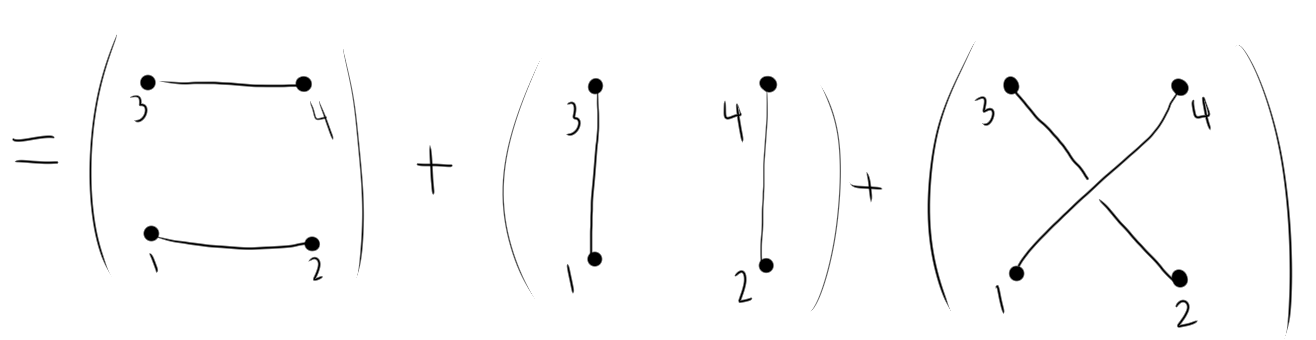
\includegraphics[scale=0.5]{images/feynman4point.png}
	\caption{Feynman diagram correspondence  of the 4-point correlation function}
\end{figure}

\noindent Keeping only unique terms, the proprotionality relation becomes an equivalence

\begin{equation}
\langle x_{j_1} \dots x_{j_l} \rangle  = \sum_{\text{unique} \,\pi^{-1}} [\textbf{A}^{-1}]_{ j_{\pi^{-1}(1)}j_{\pi^{-1}(2)}} \dots [\textbf{A}^{-1}]_{j_{\pi^{-1}(l-1)}j_{\pi^{-1}(l)}} 
\end{equation}

\noindent (\textbf{Exercise}) Calculate the 6-point correlation function with $\frac{6!}{2! 2! 2!} = 90$ unique terms

\begin{equation}
\langle x_{j_1} x_{j_2} x_{j_3} x_{j_4} x_{j_5} x_{j_6} \rangle = [\textbf{A}^{-1}]_{j_1 j_2} [\textbf{A}^{-1}]_{j_3 j_4}  [\textbf{A}^{-1}]_{j_5 j_6} + \dots
\end{equation}

\noindent In short summary,

\begin{itemize}
\item We can calculate \textit{all} moments for the Gaussian probability distribution.
\item We have a diagrammatic calculus to calculate the $l$-point correlation functions, which end up being exactly the Feynman propagators/diagrams, with appropriate choice of $\textbf{A}$, and is the direct connection of quantum field theory and Gaussian integrals.
\end{itemize}

\subsection*{The Matrix \textbf{A} for Path Integrals}

\noindent Let the potential $V$ be quadratic in the canonical position coordinate per particle $q_k$ (e.g., a one-dimensional chain of oscillators), such that the transition amplitude, which will be discretized, evaluated, and limited $\epsilon \rightarrow 0$, from some state $q_a$ to another $q_b$ is

\begin{equation}
U(q_a, q_b; T) = \left( \prod_k \int \frac{dq_k}{c(\epsilon)} \right) e^{\frac{1}{2} i q^T \textbf{A} q}
\end{equation}

\noindent Where we know the quadratic form contains a kinetic energy term plus a potential energy term

\begin{equation}
q^T \textbf{A} q = \sum_k \left( m \frac{(q_{k+1} - q_k}{\epsilon}^2 - \epsilon V (\frac{q_{k+1} + q_k}{2}) \right).
\end{equation}

\noindent This results is $\textbf{A}$ as a \textit{tridiagonal} matrix for the kinetic energy term and a potential energy term which is a matrix with elements quadratic in $q$

\begin{equation}
\textbf{A} = 
\begin{bmatrix}
    \frac{2m}{\epsilon} & -\frac{m}{\epsilon} & 0 & \cdots & & & \\
    -\frac{m}{\epsilon} & \frac{2m}{\epsilon} & -\frac{m}{\epsilon} & 0 & \cdots & & \\
    0 & -\frac{m}{\epsilon} & \frac{2m}{\epsilon}& -\frac{m}{\epsilon}& 0 & \cdots \\
    \vdots & 0 &\ddots & \ddots & \ddots
\end{bmatrix}
+ [V( q^2 )]
\end{equation}

\noindent The transition amplitude is then calculated similarly to last lecture as

\begin{equation}
U(q_a, q_b; T) = \frac{ \infty \, \text{const.}}{\sqrt{\text{det}(\textbf{A})}}
\end{equation}

\noindent The infinite constant will not be a problem since the $l$-point correlation is normalized, and the same exact infinite constant will appear in the denominator and cancel the constant. So, in terms of $q_k$, the $l$-point correlation reads

\begin{equation}
\langle q_{j_1} \dots q_{j_l} \rangle \equiv \frac{\prod_k \int \frac{dq_k}{c(\epsilon)} q_{j_1} \dots q_{j_l} \,\, e^{-\frac{1}{2} i q^T \textbf{A} x}}{\prod_k \int \frac{dq_k}{c(\epsilon)} \,\, e^{-\frac{1}{2} i q^T \textbf{A} x}}.
\end{equation}

\noindent Note that with periodic boundary conditions, the elements of follow a modulo relation $\textbf{A}_{jk} = f((j-k) \, \text{mod} \, n)$, where $n$ is the number of sites/oscillators in the chain. \\

\noindent Assuming that $\textbf{A}$ is invertible, there exists a unitary matrix $Q$, such that $Q^T Q = \mathbb{I}$ and $Q^T \textbf{A} Q = D$, with diagonal matrix $D$ with the eigenvalues of $\textbf{A}$ along the diagonal. Then the determinant of $\textbf{A}$ is easy to calculate, since 

\begin{equation}
\text{det}(\textbf{A}) = \prod_{j=1}^n \lambda_j (A).
\end{equation}

\subsection*{Correlations Functions and Quantum Observables}

\noindent Consider the transition amplitude over 2-point spatial correlations

\begin{equation}
U(q_a, q_b; T) \propto \int \mathcal{D} \phi(x) \,\, \phi(x_1) \phi(x_2) e^{i \int_{-T}^T d^4 x \, \mathcal{L}(\phi)}
\end{equation}

\noindent With an expression like this, always discretize by sending $\phi(x_j) \rightarrow q_j$, evaluate the integral, and enter the contiuum limit with the boundary conditions

\begin{align}
\phi (-T, x) &= \phi_a (x) \\
\phi (T, x) &= \phi_b (x).
\end{align}

\noindent Apply the following condition, exploiting the boundary conditions, to factor the full field "integral" over the individual fields and the boundary of the field

\begin{equation}
\int \mathcal{D} \phi (x) = \int \mathcal{D} \phi_1 (x) \int \mathcal{D} \phi_2 (x) \int_{\partial \phi} \mathcal{D} \phi (x)
\end{equation}

\noindent Where the boundary $\partial \phi = \partial \phi_1 + \partial \phi_2$ is defined by 

\begin{align}
\phi_1 (x) = \phi(x_1^0, x_1) \\
\phi_2 (x) = \phi(x_2^0, x_2)
\end{align}

\noindent So, after performing the boundary integral, we introduce quantum stuff to the expression from the classical 2-point function above, for $x_2^0 > x_1^0$

\begin{align*}
U(q_a, q_b; T) \propto \int \mathcal{D} \phi_1 (x) \int \mathcal{D} \phi_2 (x) \,\, &\phi(x_1) \phi(x_2) \bra{\phi_b} e^{-i \hat{H} (T-x_2^0)} \ket{\phi_2} \\
 &\times \bra{\phi_2} e^{-i \hat{H} (x_2^0 - x_1^0)} \ket{\phi_1} \bra{\phi_1} e^{-i \hat{H} (x_1^0 + T)} \ket{\phi_a}
\end{align*}

\noindent Now, apply the Schroedinger-picture field operator to write the classical field operators in terms of quantum field operators. The formula is

\begin{equation}
\hat{\phi}_S (x) \ket{\phi_1} = \phi (x_1) \ket{\phi_1}
\end{equation}

\noindent So, the purely quantum expression for the 2-point function is

\begin{align*}
U(q_a, q_b; T) \propto\int \mathcal{D} \phi_1 (x) \int \mathcal{D} \phi_2 (x) \,\, &\bra{\phi_b} e^{-i \hat{H} (T-x_2^0)} \hat{\phi}_S (x) \ket{\phi_2} \\
 &\times \bra{\phi_2} e^{-i \hat{H} (x_2^0 - x_1^0)} \hat{\phi}_S (x) \ket{\phi_1} \bra{\phi_1} e^{-i \hat{H} (x_1^0 + T)} \ket{\phi_a}
\end{align*}

\noindent This is called the time-ordered expectation value of the field operators in the Heisenberg picture. The equation holds for $x_2^0 < x_1^0$ as well, and we can write it as

\begin{equation}
U(q_a, q_b; T) \propto \bra{\phi_b} e^{-i \hat{H} T} \mathcal{T}[ \hat{\phi}_H (x_1) \hat{\phi}_H (x_2)] e^{-i \hat{H} T} \ket{\phi_a}
\end{equation}

\noindent Now, enter the limit as $T \rightarrow \infty$, where we bring the interacting vacuum state and the normalization for the full transition amplitude (\textbf{Exercise}), and introduce the \textit{most important formula} for this course

\begin{equation}
\bra{\Omega} \mathcal{T} [ \hat{\phi}_H (x_1) \hat{\phi}_H (x_2) ] \ket{\Omega} = \lim_{T \rightarrow \infty (1-i\epsilon)} \frac{\int \mathcal{D} \phi \,\, \phi (x_1) \phi (x_2) e^{i \int_{-T}^T d^4 x \, \mathcal{L} (\phi)}}{\int \mathcal{D} \phi \,\, e^{i \int_{-T}^T d^4 x \, \mathcal{L} (\phi)}}.
\end{equation}

\noindent So, the LHS is built of purely quantum observables equal to the classical expression of path integrals! \\

\noindent This expression will end up to be the propagator, which is also the inverse of the Klein-Gordon operator, which is what we call $\textbf{A}$ in the scalar quantum field theory. \\

\noindent The solution to this is well-known for the case when $\mathcal{L}$ is quadratic in the field operators, and one can easily discretize, evaluate the Gaussian integral, and take the limit as $\epsilon \rightarrow 0$. \\

\noindent \textbf{(Exercise)} Calculate the $l$-point formula for the time-ordered expectation value of the field operators in the Heisenberg picture.

\clearpage

\section*{Lecture 4: Functional Quantization of the Scalar Field}
\label{sec: lec4}

\noindent The path integral formalism for quantization of fields is an incredibly efficient tool, but one must learn when, and when not, ot use it. Through the lectures and many examples, we'll develop an intuition for when to trust quantization via path integrals. \\

\noindent Recall the action of the scalar field $S$ with classical field operators $\phi$

\begin{equation}
S_0 = \int d^4 x \,\, \mathcal{L}_0 = \int d^4 x \,\, \left( \frac{1}{2} (\partial_\mu \phi)^2 - \frac{1}{2} m^2 \phi^2 \right).
\end{equation}

\noindent We will (1) discretize, tantamount to imposing a cutoff $\Lambda$, (2) evaluate the integrals, and (3) enter the continuum limit where $\epsilon \rightarrow 0$. Start the discretization by putting the field on a lattice (a Lorentz manifold) with spacing $\epsilon$ and then compactify the space onto a torus for periodic boundary conditions.  \\

\noindent Mathematically, we are transforming from a four-dimensional Minkowski space $\mathcal{M}^4$ to a four-domensional torus $(\mathbb{Z}/N\mathbb{Z})^4$, where $N = \frac{L}{\epsilon}$ is the number of sites, and $L$ is the total size of grid.

%\begin{figure}[H]
%	\centering
%	\includegraphics[scale=0.5]{images/compactify.png}}
%\end{figure}

\noindent Continue discretization with the field operators

\begin{align}
\phi(x) \rightarrow &\phi(x_j) \equiv q_j, \\
&x_j=\epsilon j \in \frac{L}{N} (\mathbb{Z}/N\mathbb{Z})^4.
\end{align}

\noindent And the partial derivatives are replaced for the forward difference, which is not the best method, but it's "good enough for government work"

\begin{equation}
\partial_\mu \phi (x) \rightarrow \frac{\phi(x_j + \epsilon e^\mu) - \phi(x_j)}{\epsilon}.
\end{equation}

\noindent And the space-time integral becomes a sum over the sites on the torus

\begin{equation}
\int d^4 x \, \rightarrow \epsilon^4 \sum_{j \in (\mathbb{Z}/N\mathbb{Z})^4}
\end{equation}

\noindent Now following the path integral quanitzation recipe, consider the transition amplitude in terms of the discretized action

\begin{equation}
\bra{\phi_f} U(q_i, q_f; T) \ket{\phi_i} = \int \mathcal{D} \phi \,\, e^{i S_0}
\end{equation}

\noindent Where we follwo the "algorithm" of the integral-differential operator and discretize it to a product, over the torus sites, of integrals ($N^4$ total integrals) over the field operators, the canonical position variables 

\begin{equation}
\int \mathcal{D} \phi \rightarrow \prod_j \int d \phi (x_j) \equiv \prod_j \int d q_j.
\end{equation}

\subsection*{Discretization in Momentum Space}

\noindent Thus far we have worked entirely in real (position) space. Let's Fourier transform over into momentum space to continue discretization. The Fourier transform is a unitary transformation with Jacobian equal to 1 (\textbf{Exercise}). First, the field operators transform as

\begin{equation}
\phi (x_j) = \frac{1}{V} \sum_n e^{-i k_n \cdot x_j} \phi (k_n)
\end{equation}

\noindent Where $V=L^4$ is the volume of the 4D torus. Notationally, the $k$ argument to the field operator in momentum space $\phi (k)$ will denote the Fourier transform of the field operator in real space $\phi (x)$. The wavenumber $k_n$ is discretized over the torus as

\begin{equation}
k_n = \frac{2 \pi n^\mu}{L}, \,\, n^\mu \in \mathbb{Z}/N\mathbb{Z} \,\, \text{and} \,\, |k^\mu| < \frac{\pi}{\epsilon}
\end{equation}

\noindent Note that the Fourier space field operator is complex, such that $\phi(-k) = \phi^* (k)$, and we therefore have two independent variables per field operator in momentum space: the real part $\Re \phi (k_n)$ and the imaginary part $\Im \phi (k_n)$ for positive time-component $k_n^0 > 0$.

\noindent So, in momentum space, the discretized integral-differential operator is (\textbf{Exercise})

\begin{equation}
\int \mathcal{D} \phi = \prod_{n: k_n^0 > 0} \int d \, \Re \phi (k_n) \int d \, \Im \phi (k_n).
\end{equation}

\noindent And the discretized action for the scalar field in momentum space is (\textbf{Exercise})

\begin{equation}
S_0 = - \frac{1}{V} \sum_{k_n^0 > 0} (m^2 - k_n^2) ( (\Re \phi_n)^2 + (\Im \phi_n)^2)
\end{equation}

\noindent Where $\phi_n \equiv \phi(k_n)$, and the following relation for the Kronecker delta is used to obtain this expression

\begin{equation}
\delta_{k,0} = \frac{1}{n} \sum_{j=0}^{n-1} e^{\frac{2\pi i j k}{n}}.
\end{equation}

\noindent Our expression for the path integral for the Klein-Gordon field discretized to a lattice (four-dimensional with periodic boundary conditions) is comprised of Gaussian integarls over a finite number of degrees of freedom

\begin{equation}
I_0 = \int \mathcal{D} \phi \, e^{i S_0} = \left( \prod_{k_n^0 > 0} \int d \, \Re \phi_n \int d \, \Im \phi_n \right) e^{-i \frac{1}{V} \sum_{k_n^0 > 0} (m^2 - k_n^2 ) | \phi_n |^2}.
\end{equation}

\noindent Now, onto evaluating this integral, it's just a bunch of Gaussian integrals, and we know how to solve those. We get the following, and unrestrict $k_n$ to get the second line (\textbf{Exercise}) 

\begin{align}
I_0 &= \prod_{k_n^0 > 0} \sqrt{\frac{-i \pi V}{m^2 - k_n^2}} \cdot \sqrt{\frac{-i \pi V}{m^2 - k_n^2}} \\
I_0 &=  \prod_{k_n} \sqrt{\frac{-i \pi V}{m^2 - k_n^2}}
\end{align}

\noindent Note that $k_n$ is bounded, but we have an infinity when $V \rightarrow \infty$ (continuum limit), but this integral does not yet have full operational meaning and is proportional to the transition amplitude $I_0 \propto \bra{\phi_f} U(q_i, q_f; T) \ket{\phi_i}$, and the infinities will cancel and drop out in the full expression. \\

\subsection*{Heuristic Argument for $I_0$}

\noindent As the "surface area of knowledge" we need to remember the path integral formalism is small, there is a heuristic way to obtain this result without formal discretization, etc., using the aforementioned intuition. \\

\noindent Recall the Gaussian integral whose argument is quadratic in its independent variable

\begin{equation}
\int dx \,\, e^{-x^T \textbf{A} x} = \sqrt{\frac{\pi^n}{\text{det}(\textbf{A})}} \propto (\text{det}(\textbf{A}))^{-\frac{1}{2}}
\end{equation}

\noindent For the Klein-Gordon field, consider the path integral with the Klein-Gordon operator and field operators substituted

\begin{equation}
\int \mathcal{D} \phi \,\, e^{i S} \,\, \sim  \,\, \int \mathcal{D} \phi \,\, e^{\frac{1}{2} \int d^4 x \,\, \phi(x) (-\partial^2 - m^2) \phi (x)}
\end{equation}

\noindent So, we are boldly extrapolating to say that $\textbf{A}$ is like the Klein-Gordon operator and the $x$ is like the field operator

\begin{equation}
\int d^4 x \,\, \phi (x) (-\partial^2 - m^2) \phi (x) \sim x^T \textbf{A} x.
\end{equation}

\noindent Furthermore, we say that the path integral is proportional to the determinant of the Klein-Gordon operator

\begin{equation}
\int \mathcal{D} \phi \,\, e^{i S} \,\, \propto \,\, (\text{det}(-\partial^2 - m^2))^{-\frac{1}{2}}.
\end{equation}

\subsection*{Operationally Well-Defined Quantities}

\noindent As mentioned, $I_0$ cancels for operationally well-defined quanities, such as the 2-point correlation function, a time-ordered expectation value of products of the field operators. For example, using the path integral formalism

\begin{equation}
\bra{\Omega} \mathcal{T} [ \phi (x_1) \phi (x_2) ] \ket{\Omega} = \lim_{T \rightarrow \infty (1 - i \epsilon)} \frac{\int \mathcal{D} \phi \,\, \phi(x_1) \phi(x_2) e^{i S}}{\int \mathcal{D} \phi \,\, e^{i S}}
\end{equation}

\noindent To check our bold extrapolations, calculate the discretized field operator product

\begin{equation}
\phi (x_1) \phi (x_2) = \frac{1}{V^2} \sum_m e^{-i k_m \cdot x_1} \phi_m \sum_l e^{-i k_l \cdot x_2} \phi_l
\end{equation}

\noindent So, the discretized RHS numerator of the time-ordered expectation value above is just a bunch of  independent Gaussian integrals, quadratic in its independent variables (\textbf{Exercise})

\begin{align*}
\text{numerator} &= \frac{1}{V^2} \sum_{l,m} e^{-i (k_m \cdot x_1 + k_l \cdot x_2)} \left( \prod_{k_n^0 > 0} \int d \, \Re \phi_n \int d \, \Im \phi_n  \right) \\
&\,\,\,\,\,\, \times (\Re \phi_m + i \Im \phi_m ) (\Re \phi_l + i \Im \phi_l) e^{-i\frac{1}{V} \sum_{k_n^0 > 0} (m^2 - k_n^2 ) ((\Re \phi_n)^2 + (\Im \phi_n)^2)} \\
&= \frac{1}{V^2} \sum_m e^{-i k_m \cdot (x_1 - x_2)} \left( \prod_{k_n^0 > 0} \frac{-i \pi V}{m^2 - k_n^2} \right) \frac{-i V}{m^2 - k_n^2 - i \epsilon} \\
&= \frac{1}{V^2} \sum_m e^{-i k_m \cdot (x_1 - x_2)} \cdot I_0 \cdot \frac{-i V}{m^2 - k_n^2 - i \epsilon} 
\end{align*}

\noindent Where we drastically cut down the number of integrals to evaluate, since any integrals involving products like $\Re \phi_m \cdot \Im \phi_l$ or $\Im \phi_m \cdot \Re \phi_l$ form odd integrands and evaluate to zero. The integeral will also be zero for terms where $m \ne l$ and for terms where $k_m = k_l$. Integrals where $k_m = -k_l$ will \textit{not} be zero. \\

\noindent Bringing this together, the RHS of the time-ordered expectation value has boiled down to 

\begin{align}
\bra{\Omega} \mathcal{T} [ \phi (x_1) \phi (x_2) ] \ket{\Omega} &= \lim_{T \rightarrow \infty (1 - i \epsilon)} \frac{\int \mathcal{D} \phi \,\, \phi(x_1) \phi(x_2) e^{i S}}{\int \mathcal{D} \phi \,\, e^{i S}} \\
&= \lim_{V \rightarrow \infty} -i \frac{1}{V} \sum_n \frac{e^{-i k_n \cdot (x_1 - x_2) }}{m^2 - k_n^2 - i \epsilon} \\
&= \int \frac{d^4 k}{(2\pi)^4} \, \, \frac{i e^{-i k \cdot (x_1 - x_2)}}{-m^2 + k^2 + i \epsilon} \\
\bra{\Omega} \mathcal{T} [ \phi (x_1) \phi (x_2) ] \ket{\Omega} &= D(x_1 - x_2)
\end{align}

\noindent So, the path integral formalism gives us exactly the propagator we wish to see. Note that is we were to just boldy extrapolate, without discretization, etc., we would get the same result! \\

\noindent For example,

\begin{equation}
\frac{\int \mathcal{D} \phi \,\, \phi(x_1) \phi(x_2) e^{i S}}{\int \mathcal{D} \phi \,\, e^{i S}} = \frac{(\partial^2 - m^2)^{-\frac{1}{2}} D(x_1 - x_2)}{(\partial^2 - m^2)^{-\frac{1}{2}}}
\end{equation}

\noindent Since if $\textbf{A} \sim (-\partial^2 - m^2)$ \\
Then $[ \textbf{A}^{-1}]_{jk} \sim \frac{1}{(-\partial^2 - m^2)_{x_1 x_2}} = D(x_1 - x_2)$ \\
And  $\delta^{(4)} (x-y) = (-\partial^2 - m^2) D(x-y)$. \\

\subsection*{Example: 4-point Correlation Function}

\noindent Note that all 3-point correlations are zero, since they all have odd integrands. The 4-point correlation function starts off as

\begin{equation}
\bra{\Omega} \mathcal{T} [ \phi (x_1) \phi (x_2) \phi (x_3) \phi (x_4) ] \ket{\Omega} = \lim_{T \rightarrow \infty (1 - i \epsilon)} \frac{\int \mathcal{D} \phi \,\, \phi(x_1) \phi(x_2) \phi(x_3) \phi(x_4) e^{i S}}{\int \mathcal{D} \phi \,\, e^{i S}}.
\end{equation}

\noindent The numerator contains the quantities of $(\Re \phi_m + i \Im \phi_m) \dots (\Re \phi_l + i \Im \phi_l)$, and most terms will vanish as before, leaving us with terms where $k_l = -k_m$ and $k_q = -k_p$, and we end up with, after applying Wick's theorem and sending $V \rightarrow \infty$ (\textbf{Exercise}), something like

\begin{align*}
&\sum_{k_l, k_q} e^{-i \dots} \int \dots \phi_{k_l} \phi_{-k_l} \phi_{k_q} \phi_{-k_q} e^{\dots} \\
&= D_F(x_1 - x_2) D_F (x_3 - x_4) + D_F (x_1 - x_3) D_F (x_2 - x_4) + D_F (x_1 - x_4) D_F (x_2 - x_3)
\end{align*}

\subsection*{Interacting QFT via Path Integrals}

\noindent Consider the action with a free part and an interacting part, namely the phi-fourth interaction,

\begin{equation}
S = S_0 + S_{int} = S_0 + \frac{i \lambda}{4!} \int d^4 x \,\, \phi^4 (x).
\end{equation}

\noindent Then the time-ordered expectation value for 2-point correlations can be Taylor expanded, since $\lambda$ is small,

\begin{align}
\bra{\Omega} \mathcal{T} [ \phi (x_1) \phi (x_2) ] \ket{\Omega} &= lim_{T \rightarrow \infty (1 - i \epsilon)} \frac{\int \mathcal{D} \phi \,\, \phi(x_1) \phi(x_2) e^{i (S_0 + S_{int})} }{\int \mathcal{D} \phi \,\, e^{i (S_0 + S_{int})}} \\
&= lim_{T \rightarrow \infty (1 - i \epsilon)} \frac{\int \mathcal{D} \phi \,\, \phi(x_1) \phi(x_2) e^{i S_0} (1 + S_{int} + \frac{1}{2} S_{int}^2 + \dots)}{\int \mathcal{D} \phi \,\, e^{i S_0} (1 + S_{int} + \frac{1}{2} S_{int}^2 + \dots)}
\end{align}

\noindent Where $S_{int} = \frac{i \lambda}{4!} \int d^4 z \,\, \phi^4 (z)$, and each term above is an integral of powers of time-ordered quantum field operators which end up as Feynman diagrams, for example, of the form

\begin{align}
&\frac{\lambda^m}{4!^m} \int d^4 z_1 \dots \int d^4 z_m \int \mathcal{D} \phi \,\, \phi(x_1) \phi(x_2) \phi^4(z_1) \dots \phi^4(z_m) e^{i S_0} \\
&= \frac{\lambda^m}{4!^m} \int d^4 z_1 \dots \int d^4 z_m \bra{\Omega} \mathcal{T} [\hat{\phi}(x_1) \hat{\phi}(x_2) \hat{\phi}^4 (z_1) \dots \hat{\phi}^4 (z_m) ] \ket{\Omega} \\
&= \text{Sum of Feynman diagrams}
\end{align}

\clearpage

\section*{Lecture 5: Functional Derivatives and Generating Functionals}
\label{sec: lec5}


\noindent Here we will finish the functional quantization of the scalar field. \\

\noindent Recall that we can compute time-ordered correlation functions for the quantum scalar field entirely in terms of classical quantities, which is equivalent to a sum over all diagrams,

\begin{equation}
\bra{\Omega} T[ \hat{\phi} (x_1) \dots \hat{\phi} (x_n) ] \ket{\Omega} = \lim_{T \rightarrow \infty(1-i\epsilon)} \frac{\int \mathcal{D} \phi \,\, \phi(x_1) \dots \phi(x_n) e^{i S[\phi(x_1), \dots , \phi (x_n)]}}{\int \mathcal{D} \phi \,\, e^{i S[\phi(x_1), \dots , \phi (x_n)]}}
\end{equation}

\noindent For example, the 2-point correlation function for the Klein-Gordon field is the Feynman propagator

\begin{equation}
\bra{\Omega} T[ \hat{\phi} (x_1) \hat{\phi} (x_2) ] \ket{\Omega} = \lim_{T \rightarrow \infty(1-i\epsilon)} \frac{\int \mathcal{D} \phi \,\, \phi(x_1) \phi(x_2) e^{i S}}{\int \mathcal{D} \phi \,\, e^{i S}} = D_F (x_1 - x_2)
\end{equation}

\noindent More elegantly, and analogous to multivariate Gaussian integrals, we found the Feynman propagator $D_F (x-y)$, which is the inverse operator of the Klein-Gordon operator $-\partial^2 - m^2$, to be similiar to the inverse of a matrix $\textbf{A}$, making the Klein-Gordon operator the matrix $\textbf{A}$. 

\begin{equation}
D_F (x_j - x_k) \sim [\textbf{A}^{-1}]_{jk} = \frac{\int dx_1 \dots dx_n \,\, x_j x_k e^{-\frac{1}{2} x^T \textbf{A} x} }{\int dx_1 \dots dx_n \,\, e^{-\frac{1}{2} x^T \textbf{A} x}}
\end{equation}

\noindent To compute these $n$-point correlation functions, or elements of this "inverse matrix", we used derivatives of the generating functional, which is what we generalize in this lecture. Recall the multivariate Gaussian generating functional

\begin{equation}
Z[J] = \int dx_1 \dots dx_n e^{ -\frac{1}{2} x^T \textbf{A} x - J^T x } = e^{ \frac{1}{2} J^T \textbf{A}^{-1} J }.
\end{equation}

\subsection*{Functional Derivatives}

\noindent The functional derivative is a tool from the calculus of variations that we now define by an example that is the continuum analog of the standard partial derivative

\begin{equation}
\frac{\delta}{\delta J(x)} J(y) = \delta^{(4)} (x-y).
\end{equation}

\noindent There is a \textit{one-to-one} mapping from the discrete representation to the continuous with correspondences

\begin{equation}
\begin{array}{ccc}
x \in \mathbb{R} & \rightarrow & j \in \mathbb{Z} \\
J(x) \in C(\mathbb{R}) & \rightarrow & J_j \in L_2(\mathbb{Z}) \\
\frac{\delta}{\delta J(x)} F[J(y)] & \rightarrow & \frac{\partial}{\partial J_j} F[J_1, J_2, \dots]
\end{array}
\end{equation}

\noindent Where $C(\mathbb{R})$ is a continuous function space and $L_2(\mathbb{Z})$ is ...

\subsubsection*{Example 1}

\begin{align*}
\frac{\delta}{\delta J(x)} e^{i \int d^4 y \, J(y) \phi (y)} &= i e^{i \int d^4 y \, J(y) \phi (y)} \frac{\delta}{\delta J(x)} \left( \int d^4 y \, J(y) \phi (y) \right) \\
&= i e^{i \int d^4 y \, J(y) \phi (y)} \int d^4 y \, \frac{\delta J(y)}{\delta J(x)} \phi(y) \\
&= i e^{i \int d^4 y \, J(y) \phi (y)} \int d^4 y \, \delta^{(4)} (x-y) \phi(y) \\
\frac{\delta}{\delta J(x)} e^{i \int d^4 y \, J(y) \phi (y)} &= i \phi (x) e^{i \int d^4 y \, J(y) \phi (y)}
\end{align*}

\subsubsection*{Example 2: Derivatives of Delta functions}

\begin{align*}
\frac{\delta}{\delta J(x)} \int d^4 y \, (\partial_\mu J(y) ) v^\mu (y) &= \frac{\delta}{\delta J(x)} \left( \text{boundary term}  - \int d^4 y \, J(y) \partial_\mu v^\mu (y) \right) \\
&= -\partial_\mu v^\mu (x)
\end{align*}

\noindent Note that the boundary term is almost always zero, except for topologically interesting theories.

\subsection*{The Generating Functional}

\noindent Define the generating functional as

\begin{equation}
Z[J] = \lim_{T \rightarrow \infty(1-i \epsilon)} \int \mathcal{D} \phi \,\, e^{i S + i J(x) \phi(x)}.
\end{equation}

\noindent This expression is obviously useful, since correlation functions are directly related to derivatives of $Z[J]$

\begin{equation}
\bra{\Omega} T [ \hat{\phi} (x) \hat{\phi} (y) ] \ket{\Omega} = \frac{- \frac{\delta}{\delta J(x)}  \frac{\delta}{\delta J(y)} Z[J] \big{|}_{J=0}}{Z[J] \big{|}_{J=0}}
\end{equation}

\noindent So, if you can compute the generating functional $Z[J]$, you have \textit{all} of the $n$-point correlation functiosn via derivatives for your field theory. \\

\noindent In free field theories, such as the Klein-Gordon field, the action is quadratic in the field operators, and the argument of the exponential is $Z[J]$ is

\begin{equation}
i(S_0 + J(x) \phi (x) = i \int d^4 x \,\, \left( \frac{1}{2} \phi (x) (-\partial^2 - m^2 + i \epsilon) \phi (x) + J(x) \phi(x) \right).
\end{equation}

\noindent To homogenize quadraticity, complete the square by introducing the shift (with Jacobian $=1$

\begin{equation}
\phi' (x) = \phi (x) - i \int d^4 y \,\, D_F (x-y) J (y).
\end{equation}

\noindent This is analogous to the positional shift $x' = x - \textbf{A}^{-1} J$, and works becuase the Feynman propagator is the inverse of the Klein-Gordon operator, such that 

\begin{equation}
(-\partial^2 - m^2 ) D_F (x-y) = i \delta^{(4)} (x-y)
\end{equation}

\noindent With the variable change, the exponential argument becomes

\begin{align*}
i(S_0 + J(x) \phi (x) = & i \int d^4 x \,\, \left( \frac{1}{2} \phi' (x) (-\partial^2 -m^2 + i \epsilon) \phi' (x) \right) \\
&- i \int d^4 x \int d^4 y \, \left( \frac{1}{2} J(x) (-i D_F (x-y)) J(y) \right).
\end{align*}

\noindent So, the generating functional is then

\begin{equation}
Z[J] = Z_0 e^{-\frac{1}{2} \int d^4 x d^4 y \, ( J(x) D_F (x-y) J (y))}
\end{equation}

\noindent Where the free field contribution, independent of $J$, is

\begin{equation}
Z_0 = \int \mathcal{D} \phi' \,\, e^{ i \int d^4 x \,\, \left( \frac{1}{2} \phi' (x) (-\partial^2 -m^2 + i \epsilon) \phi' (x) \right)}.
\end{equation}

\subsubsection*{Examples of Free Theory Correlations Functions}

\noindent \textbf{Example 1:} The 2-point correlation function, with the $Z_0$ cancelled out,

\begin{equation}
\bra{\Omega} T [ \hat{\phi} (x) \hat{\phi} (y) ] \ket{\Omega} = - \frac{\delta}{\delta J(x)}  \frac{\delta}{\delta J(y)} e^{-\frac{1}{2} \int d^4 x d^4 y \, ( J(x) D_F (x-y) J (y))} \big{|}_{J=0}.
\end{equation}

\noindent \textbf{Example:} The 4-point correlation function, with notation $\hat{\phi}_i = \hat{\phi} (x_i)$, $J_i = J (x_i)$, and $D_{xi} = D(x - x_i)$

\begin{align}
\bra{0} T[ \hat{\phi_1} \hat{\phi}_2 \hat{\phi}_3 \hat{\phi}_4 ] \ket{0} &= \frac{ \frac{\delta}{\delta J_1} \frac{\delta}{\delta J_2} \frac{\delta}{\delta J_3} \frac{\delta}{\delta J_4}  Z[J] \big{|}_{J=0} }{ Z[J=0] } \\
&= \frac{\delta}{\delta J_1} \frac{\delta}{\delta J_2} \frac{\delta}{\delta J_3} \left( - \int d^4 x' \,\, J_{x'} D_{x' 4} e^{-\frac{1}{2} \int d^4 x \int d^4 y J_x D_{xy} J_y} \right) \big{|}_{J=0}  \\
&= \frac{\delta}{\delta J_1} \frac{\delta}{\delta J_2} \left( -D_{34} + \int d^4 x' \int d^4 y' \, J_{x'} D_{x' 3} J_{y'} D_{y' 4} \right) \times e^{\dots} \big{|}_{J=0}   \\
&= \frac{\delta}{\delta J_1} \left( D_{34} \int d^4 x' \, J_{x'} D_{x' 2} + D_{24} \int d^4 y' \, J_{y'} D_{y' 3} + D_{23} \int d^4 z' \, J_{z'} D_{z' 4} + \mathcal{O} (J^2) \right) e^{\dots} \big{|}_{J=0}  \\
&= D_{34} D_{12} + D_{24} D_{13} + D_{23} D_{14}
\end{align}

\subsubsection*{Interacting Fields}

\noindent The time-ordered expectation value, which contains the generating functions by Taylor expansion, for the (classical) phi-fourth interacting theory is 

\begin{equation}
\bra{\Omega} T[ \phi_1 \dots \phi_n] \ket{\Omega} = \lim_{T \rightarrow \infty (1-i \epsilon )} \frac{ \int \mathcal{D} \, \phi e^{i(S_0 + S_{int})} \phi (x_1) \dots \phi (x_n) }{\int \mathcal{D} \phi \, e^{i(S_0 + S_{int})}}
\end{equation}

\noindent Where $S_{int} = -\frac{i \lambda}{4!} \int d^4 x \, \phi^4 (x)$. \\

\subsubsection*{Fermionic Fields}

\noindent For the (classical) \textit{fermionic field} $\hat{\psi}$, the 2-point correlation function, vacuum expectation value, is

\begin{equation}
\bra{\Omega} T[ \psi (x) \psi (y)] \ket{\Omega} = \frac{ \int \mathcal{D} \, \psi e^{iS} \psi (x) \psi (y) }{\int \mathcal{D} \psi \, e^{iS}}
\end{equation}

\noindent Rule number one for this expression (1) is to not think abou this operationally, and rule number two (2) is to think in analogy to complex numbers, which can provide a more clear representation and make things easier.  \\

\noindent The Fermi fields obey the relations

\begin{align}
\psi^2 (x) &= 0 \\
\psi (x) \psi (y) &= - \psi (y) \psi (x)
\end{align}

\subsection*{Vignette: Anticommuting Numbers (Grassman Numbers)}

\noindent Let $V$ be an $n$-dimensional vector space with basis $\theta_a \in V$, $a=1,\dots,n$. Thus, elements of the vector space $v \in V$ have the form 

\begin{equation}
v = \sum_{a=1}^n v_a \theta_a.
\end{equation}

\noindent To build a bigger vector space $\mathcal{G}(V)$ from $V$, we first endow $V$ with the product operation denoted by concatenation (e.g., $\theta_a \cdot \theta_b \cdot \theta_c = \theta_a \theta_b \theta_c$). \\

\noindent This gives us an infinite dimensional vector space with span

\begin{equation}
\mathcal{S}^{\infty} (V) = \text{span} \{ \theta_a, \theta_a \theta_b, \theta_a \theta_b \theta_c, \dots \}
\end{equation}

\noindent Now restrict the basis to obey the following suggestive relations

\begin{align}
\theta_a \theta_b &= - \theta_b \theta_a \\
\theta_a^2 &= 0.
\end{align}

\noindent Then the new vector space has dimension $\text{dim}(\mathcal{G} (V)) = 2^n$, and is the infinite dimensional span modulo the elements of the underlying vector space

\begin{equation}
\mathcal{G}(V) = \mathcal{S}^{\infty} (V) / v.
\end{equation}

\noindent (\textbf{Exercise}) Check that this structure is well-defined. Note that this is exactly the space of differential forms for a tangent space $V$ (also known as the space of "classical fermions"). \\

\noindent The basis of $\mathcal{G} (V)$ is now 

\begin{equation}
\{ 1, \, \theta_a, \, \theta_a \theta_b, \, \theta_a \theta_b \theta_c, \dots \}
\end{equation}

\noindent With $a=1,\dots,n$, followed by $1 \le a < b \le n$, $a < b < c$, etc. \\

\noindent Then a general element of the new vector space $f \in \mathcal{G} (V)$ is

\begin{align}
f = \alpha + \sum_{p=1}^n \,\, \sum_{1 \le j_1 < \dots < j_p \le n} \alpha_{j_1 j_2 \dots j_p} \, &\theta_{j_1} \theta_{j_2} \dots \theta_{j_p} \\
&, \text{where} \,\, \alpha_{j_1 j_2 \dots j_p} \in \mathbb{C}.
\end{align}

\clearpage

\section*{Lecture 6: Grassmann Numbers}
\label{sec: lec6}


\noindent We left off with an object meant to be the classical version of a fermion: a Grassman number. It is the object of a vector space $ \mathcal{G}_n (V)$, generated by basis $\{ 1, \theta_1, \dots, \theta_n \in V \}$. Imposing the anticommutation relation 

\begin{equation}
\{\theta_j, \theta_k \} = 0, \, \forall j,k = 1, \dots, n
\end{equation}

\noindent This is a $2^n$-dimensional vector space with monomial basis

\begin{equation}
\{ 1, \theta_1, \theta_2, \dots, \theta_n, \theta_1 \theta_2, \dots , \theta_{n-1} \theta_n, \dots , \theta_1 \theta_2 \dots \theta_n \}.
\end{equation}

\noindent An arbitrary element $f \in \mathcal{G}_n (V)$

\begin{equation}
f = f_0 + \sum_{j_1 < \dots < j_p} f_p (j_1, \dots , j_p) \, \theta_{j_1} \dots \theta_{j_p}
\end{equation}

\noindent We now define functions, linear and nonlinear, representations, complex numbers, calculus, derivatives, and integrals of Grassman numbers.

\subsection*{Functions of Grassman Numbers}

\noindent Think of $\theta_j$ as anticommuting numbers/variables. \\

\noindent Note: A "wrong" definition is to let $f$ be an infinitely differentiable function $f \in C^\infty (\mathbb{R})$, adjoin the symbol $f(\theta_j)$, and impose the anticommutation relation $\{ f(\theta_j), \theta_k \} = 0, \, \forall \, j, k$. Then each $f$ will produce a new anticommuting object, which leads to an uncountably infinite number of objects, and is not what we expect from a function. \\

\noindent Linear functions should be linear maps from the vector space to itself, $F \in \mathcal{M}_{2^n} (\mathbb{C})$, the space of $2^n \times 2^n$ matrices

\begin{equation}
F : \,\, \mathcal{G}_n (V) \rightarrow \mathcal{G}_n (V)
\end{equation}

\noindent Nonlinear functions will be defined by analogy to the functional calculus of matrices; consider a matrix $M \in \mathcal{M}_m (\mathbb{C})$. As long as $M$ is diagonalizable, define the nonlinear function $f(M) = S^{-1} f(D) S$, where $M$ is diagonalized by S, such that $M = S^{-1} D S$. Since a diagonal matrix occupies a commutative algebra, we know how to define function for $D$ and then rotate from $D$ to $M$ via $S$. \\

\noindent In summary so far, one strategy to define functions of Grassman numbers is to represent $\mathcal{G}_n (V)$ as matrices and use functional calculus. Working with representations, we now need matrices to represent the Grassman numbers.

\subsection*{Representations of $\mathcal{G}_n (V)$}

\noindent Consider a map from our vector space to a concrete space of matrices

\begin{equation}
\pi : \,\, \mathcal{G}_n (V) \rightarrow M_d (\mathbb{C}
\end{equation}

\noindent Which must obey the anticommutation relation

\begin{equation}
\{ \pi (\theta_j), \pi (\theta_k) \} = 0, \,\, \forall j,k .
\end{equation}

\noindent Construct the "Jordan-Wigner representation", which will look very familiar. Begin with a Hilbert space $\mathcal{H} = \mathbb{C}^{2^n}$, with dimension $2^n$, and Pauli operators 

\begin{align}
\sigma^+ &= \left( \begin{matrix} 0 & 0 \\ 1 & 0 \end{matrix}  \right) \\
\sigma^z &= \left( \begin{matrix} 1 & 0 \\ 0 & -1 \end{matrix} \right).
\end{align}

\noindent Recall that these Pauli operators obey the relations

\begin{align}
\{ \sigma^+ , \sigma^z \} &= 0 \\
(\sigma^+ )^2 &= 0.
\end{align}

\noindent Construct the representation of $\mathcal{G}_n (V)$

\begin{align}
\pi (\theta_1 ) &= \sigma_1^+ \otimes \mathbb{I}_2 \otimes \dots \otimes \mathbb{I}_{n-1} \otimes \mathbb{I}_n \\
\pi (\theta_2 ) &= \sigma_1^z \otimes \sigma_2^+ \otimes \dots \otimes \mathbb{I}_{n-1} \otimes \mathbb{I}_n \\ 
&\dots \\
\pi (\theta_n) &= \sigma_1^z \otimes \sigma_2^z \otimes \dots \otimes \sigma_{n-1}^z \otimes \sigma_n^+
\end{align}

\subsubsection*{Single variable representation ($n=1$)}

\noindent Let $F \in C^\infty (\mathbb{R}, \mathbb{R})$ and $\mathcal{G}_1 (V) \simeq \{ a+b \theta : \, a,b \in \mathbb{C} \}$. This should be consistent with the functional calculus of the representation $\pi(\cdot)$, such that $F(\pi(\cdot)) = S^{-1} F(D) S$. 

\noindent To evaluate the function $F$, we write out the Taylor series, evaluate at $x=\theta$, and impose the defined relations (e.g., $\theta_j^2 = 0, \, \forall j$)

\begin{align}
F(x) &= \sum_{j=0}^\infty \frac{F^{(j)} (x=0) x^j}{j!} \\
F(\theta) &= \sum_{j=0}^\infty \frac{F^{(j)} (\theta=0) \theta^j}{j!} \\
F(\theta) &= F^{(0)} (\theta=0) + F^{(1)} (\theta=0) \cdot \theta
\end{align}

\textbf{Example 1:}

\begin{align}
F(x) &= \sin(x) \\
F(\theta) &= (x - \frac{x^3}{3!} + \dots ) \big{|}_{x=\theta} \\
F(\theta) &= \theta
\end{align}

\textbf{Example 2: }

\begin{equation}
F(x) = x + x^3 \rightarrow F(\theta) = \theta
\end{equation}

\subsubsection*{Multiple variable representation}

\noindent Let $F \in C^\infty (\mathbb{R}^n, \mathbb{R})$, with the Taylor expansion

\begin{equation}
F(\theta_1, \dots , \theta_n) = F^{(0)} (\theta_1=0, \dots , \theta_n=0) + \sum_{j=1}^n \theta_j \frac{\partial F(0, \dots , 0)}{\partial \theta_j} + \mathcal{O}(\theta^2)
\end{equation}

\textbf{Example 1: $n=2$}

\begin{align}
F(x,y) &= e^{-\lambda x y} \\
F(\theta_1, \theta_2) &= (1 - \lambda x y + \lambda^2 x^2 y^2 + \dots ) \big{|}_{x=\theta_1, y=\theta_2} \\
F(\theta_1, \theta_2) &= 1 - \lambda \theta_1 \theta_2
\end{align}

\textbf{Example 2: $n=2$}

\begin{align}
F(x,y) &= e^{-\lambda_1 x - \lambda_2 y} \\
F(\theta_1, \theta_2) &= (1 - \lambda_1 \theta_1 ) ( 1 - \lambda_2 \theta_2) \\
F(\theta_1, \theta_2) &= 1 - \lambda_1 \theta_1 - \lambda_2 \theta_2 + \lambda_1 \lambda_2 \theta_1 \theta_2
\end{align}

\noindent Note that even though we lose higher order terms such as $\theta_j^2$, nonlinear features are preserved in the multivariable case.

\subsubsection*{Complex Grassman Numbers}

\noindent Let $\theta_1$, $\theta_2 \in \mathcal{G}_2 (V)$, a 4-dimensional vector space with basis $\{1, \theta_1, \theta_2, \theta_1 \theta_2 \}$, and define the quantities $\theta$ and $\theta^* \in \mathcal{G}_2 (V)$ as

\begin{align}
\theta &= \frac{\theta_1 + i \theta_2}{\sqrt{2}} \\
\theta^* &= \frac{\theta_1 - i \theta_2}{\sqrt{2}}.
\end{align}

\noindent To extend to the multivariable case, define

\begin{equation}
\theta_j^* = \frac{\theta_{j_1} - i \theta_{j_2}}{\sqrt{2}}
\end{equation}

\noindent Where $\theta_{j_1}, \, \theta_{j_2} \in \mathcal{G}_{2n} (V)$.

\subsubsection*{Grassman Derivatives}

\noindent Define the derivative with respect to Grassman variables as the map

\begin{equation}
\partial_{\theta_j} : \,\, \mathcal{G}_n (V) \rightarrow \mathcal{G}_n (V)
\end{equation}

\noindent Which obeys the relations

\begin{enumerate}
\item $\partial_{\theta_j} (\theta_k) = \delta_{jk}$
\item $\partial_{\theta_j} (\theta_{k_1} \dots \theta_{k_p}) = \delta_{j k_1} \theta_{k_2} \dots \theta_{k_p} - \delta_{j k_2} \theta_{k_1} \theta_{k_3} \dots \theta_{k_p} + \dots + (-1)^{p-1} \delta_{j k_p} \theta_{k_1} \dots \theta_{k_{p-1}}$.
\end{enumerate}

\noindent The second relation follows from the anticommutation relation, and can be thought of as bringing the corresponding $\theta_j$ to the front via anticommutations and then differentiating. \\
\noindent For example,

\begin{equation}
\partial_{\theta_2} (\theta_1 \theta_2 ) = - \partial_{\theta_2} (\theta_2 \theta_1) = - \theta_1.
\end{equation}

\noindent (\textbf{Exercise}) These relations can be extended by linearity for any Grassman number. This definition of $\partial_{\theta_j}$ obeys the product rule and the chain rule.

\subsubsection*{Grassman Integrals}

\noindent Following the analogy of the common definite integral, the Grassman integral should be a linear map which obeys shift invariance, such that $\theta \rightarrow \theta + \eta$,

\begin{equation}
\int d\theta : \,\, \mathcal{G}_n (V) \rightarrow \mathbb{C}.
\end{equation}

\noindent The only consistent definition to satisfy these two constraints for a single Grassman variable is 

\begin{equation}
\int d\theta \,\, (a + b \theta) = b, \,\, a,b \in \mathbb{C}
\end{equation}

\noindent Note the very interesting property here that, by this definition, the integral and the derivative are the exact same thing

\begin{equation}
\int d\theta \, (a + b \theta) = \partial_\theta (a + b \theta).
\end{equation}

\noindent This also holds for the multivariable case, where the highest order term is picked off from the Taylor series

\begin{equation}
\int d\theta_n \dots d\theta_1 \, (f_0 + \sum_{j_1 < \dots < j_p} f_p (j_1, \dots, j_p) \theta_{j_1} \dots \theta_{j_p}) = f_n (1, \dots, n).
\end{equation}

\noindent This is a weird definition, but it works, behaves correctly under change of variables, and does what we need it to do. \\

\textbf{Example:}  $n=2$ independent Grassman numbers

\begin{align}
\int d\theta^* d\theta \, e^{-\lambda \theta^* \theta} &= \int d\theta^* d\theta \, (1-\lambda \theta^* \theta) \\
&= \partial_{\theta^*} \partial_\theta \, (1 - \lambda \theta^* \theta) \\
\int d\theta^* d\theta \, e^{-\lambda \theta^* \theta} &= \lambda
\end{align}

\noindent Note that the order of integration ($\theta$ first, $\theta^*$ second) is by convention.

\subsubsection*{Multivariable Gaussian Integrals}

\noindent Consider the multivariable Gaussian integral

\begin{equation}
I = \int d\theta_1^* d\theta_1 \dots d\theta_n^* d\theta_n \,\, e^{-\sum_{j,k} \theta^*_j B_{jk} \theta_k}
\end{equation}

\noindent Where $B^\dagger = B$ and we diagonalize via $U^\dagger B U = D$. \\

\noindent Make a change of variables $\theta'_j = U_{jk} \theta_k$, where $U$ is a unitary matrix, such that the product of these new Grassman variables is (\textbf{Exercise})

\begin{align}
\theta'_1 \theta'_2 \dots \theta'_n &= \sum_{k_1, \dots, k_n} U_{1 k_1} U_{2 k_2} \dots U_{n k_n} \theta_{k_1} \theta_{k_2} \dots \theta_{k_n} \\
&= \sum_{\pi \in S_n} U_{1 \pi(1)} \dots U_{n \pi(n)} \text{sgn}(\pi) \theta_1 \theta_2 \dots \theta_n \\
\theta'_1 \theta'_2 \dots \theta'_n &= \text{det} (U) \theta_1 \theta_2 \dots \theta_n
\end{align}

\noindent So the Gaussian integral becomes

\begin{align}
I &= \int d{\theta'}_1^* d\theta'_1 \dots d{\theta'}_n^* d\theta'_n \,\, e^{-\sum_{j,k} {\theta'}^*_j (U B U^\dagger )_{jk} \theta'_k} \text{det}(U) \text{det}(U^\dagger) \\
&= \int d{\theta'}_1^* d\theta'_1 \dots d{\theta'}_n^* d\theta'_n \,\, e^{-\lambda_1 {\theta'}_1^* \theta'_1} \dots e^{-\lambda_n {\theta'}_n^* \theta'_n} \cdot (1) \cdot (1) \\
&= \lambda_1 \lambda_2 \dots \lambda_n \\
I &= \text{det} (B)
\end{align}

\noindent Recall that for the normal Gaussian integral case, we got $I = (\text{det}(B))^{-1}$. \\

\noindent (\textbf{Exercise}) The generating functional for the Grassman calculus is, where $J$ is a vector of Grassman numbers,

\begin{align}
Z [J] &= \int d\theta_1^* d\theta_1 \dots d\theta_n^* d\theta_n \,\, e^{-\theta^\dagger B \theta + J^\dagger \theta + \theta^\dagger J} \\
&= e^{J^\dagger B^{-1} J}.
\end{align}

\noindent The moments are (\textbf{Exercise})

\begin{equation}
\int d\theta_1^* d\theta_1 \dots d\theta_n^* d\theta_n \,\, \theta_j \theta_k^* e^{-\theta^\dagger B \theta} = \text{det} (B) \cdot [B^{-1}]_{jk}
\end{equation}

\noindent \textbf{Side}: The mixing of regular and Grassman numbers provides the basis for the supersymmetric method. Consider the Gaussian integral

\begin{align}
\int d \Phi e^{-\Phi^\dagger M \Phi} &= \int dx_1 \dots dx_n dx_1^* \dots dx_n^* \int d\theta_1^* d \theta_1 \dots d \theta_n^* d \theta_n \, e^{-\Phi^\dagger M \Phi} \\
&= (\text{det} A)(\text{det} A)^{-1} \\
\int d \Phi e^{-\Phi^\dagger M \Phi} &= 1
\end{align}

\noindent Where $\Phi = (x_1, \dots, x_n, \theta_1, \dots, \theta_n)$ and $M$ is a $2n \times 2n$ matrix

\begin{equation}
M= \left( \begin{matrix} A & 0 \\ 0 & A \end{matrix}  \right)
\end{equation}

\clearpage

\section*{Lecture 7: Functional Quantization of the Dirac Field}
\label{sec: lec7}

\noindent We now employ Grassmann numbers/variables to build a path integral-like object that provides the $n$-point correlation functions for the Dirac (spinor) field. \\

\noindent Consider the Grassmann integral of the complex Grassmann variables $\theta$ and $\theta^*$, the Grassmann Gaussian generating function

\begin{equation}
Z[J] = \left( \prod_{j=1}^n \int d\theta^*_j d\theta_j \right) e^{- \sum_{j,k} \theta_j^* B_{jk} \theta_k + \sum_j (J_j^* \theta_j + \theta^*_j J_j) }
\end{equation}

\noindent Where the Grassmann variables and auxiliary fields $J$ and $J^*$ obey the anticommutation relations

\begin{align}
\{ \theta_j, \theta_k^* \} &= \{ \theta_j, \theta_k \} = \{\theta_j^*, \theta_k^* \} = 0 \\
\{J_j, \theta_k \} &= \{J_j^*, \theta_k \} = \{ J_j, J_k^* \} = 0.
\end{align}

\noindent Calculating these Gaussian integrals, the generating functional becomes

\begin{equation}
Z[J] = e^{- \sum_{j,k} J_j^* [B^{-1}]_{jk} J_k}.
\end{equation}

\noindent Since the matrix $B$ is unitary, such that $B^\dagger = B$, the generating functional $Z[J]$ is Hermitian. \\

\noindent Note that the generating functional takes a vector of Grassmann numbers, anticommuting objects, as input and yields an expression quadratic in the Grassmann numbers which evaluates to a real number, a commuting object, since observables correspond to Hermitian operators and real numbers as their eigenvalues; the expectation value must always be a real number, not a Grassmann number.

%
\noindent We now employ Grassmann numbers/variables to build a path integral-like object that provides the $n$-point correlation functions for the Dirac (spinor) field. \\

\noindent Consider the Grassmann integral of the complex Grassmann variables $\theta$ and $\theta^*$, the Grassmann Gaussian generating function

\begin{equation}
Z[J] = \left( \prod_{j=1}^n \int d\theta^*_j d\theta_j \right) e^{- \sum_{j,k} \theta_j^* B_{jk} \theta_k + \sum_j (J_j^* \theta_j + \theta^*_j J_j) }
\end{equation}

\noindent Where the Grassmann variables and auxiliary fields $J$ and $J^*$ obey the anticommutation relations

\begin{align}
\{ \theta_j, \theta_k^* \} &= \{ \theta_j, \theta_k \} = \{\theta_j^*, \theta_k^* \} = 0 \\
\{J_j, \theta_k \} &= \{J_j^*, \theta_k \} = \{ J_j, J_k^* \} = 0.
\end{align}

\noindent Calculating these Gaussian integrals, the generating functional becomes

\begin{equation}
Z[J] = e^{- \sum_{j,k} J_j^* [B^{-1}]_{jk} J_k}.
\end{equation}

\noindent Since the matrix $B$ is unitary, such that $B^\dagger = B$, the generating functional $Z[J]$ is Hermitian. \\

\noindent Note that the generating functional takes a vector of Grassmann numbers, anticommuting objects, as input and yields an expression quadratic in the Grassmann numbers which evaluates to a real number, a commuting object, since observables correspond to Hermitian operators and real numbers as their eigenvalues; the expectation value must always be a real number, not a Grassmann number. \\

\noindent Recall the Dirac spinor field which is what we mean to be classical fermions. The classical fermion is represented by the 4-component spacetime vector

\begin{equation}
\psi (x) \rightarrow M(\Lambda) \psi (\Lambda^{-1} x)
\end{equation}

\noindent With the representation of the Lorentz group

\begin{equation}
M = e^{-\frac{i}{2} \omega_{\mu\nu} S^{\mu \nu}}.
\end{equation}

\noindent Where $S^{\mu\nu} = \frac{i}{4} [\gamma^\mu, \gamma^\nu]$ and $\{ \gamma^\mu, \gamma^\nu \} = 2 \eta^{\mu\nu}$. An object that transforms according to the transformation law with this representation we call a Dirac spinor. The representation, and thus the generators, of the Poincar\'e group easily follows. \\

\noindent The Hamiltonian, or generator of time translations, that follows from this spinor object solves the Dirac equation $(i\partial_\mu \gamma^\mu - m) \psi = 0$. Recall that we defined the conjugate-like object $\bar{\psi} = \psi^\dagger \gamma^0$ to induce Lorentz invariance for the Lagrangian density $\mathcal{L} = \bar{\psi} (-i\slashed{\partial} - m) \psi$, where the slash notation denotes $\slashed{A} = A_\mu \gamma^\mu$. \\

\noindent Thus far, we've been thinking about $\psi = (\psi_1, \psi_2, \psi_3, \psi_4)$ as the classical spinor-valued Dirac field, but it is really the single-particle component that is needed to build the classical Dirac field with anticommuting objects, since we guess to employ the anticommutation relation of quantum Dirac field operators 

\begin{equation}
\{ \hat{\psi} (x), \hat{\psi}^\dagger (y) \} = \delta^{(4)} (x-y).
\end{equation}

\noindent So, to build a quantum theory, recall that we, in the case of creation and annihilation operators, for example,

\begin{enumerate}
\item Pick a classical single-particle theory
\item Put hats on the field operators to quantize them
\item Make an algebra for the quantized field operators to obey
\item Find representations of that algebra.
\end{enumerate}

\noindent Alternatively, we can find some classical Dirac field that we quantize via the path integral, and use the path integral as a tool to guess the quantum theory. \\

\noindent \textbf{Guess 1 (Wrong):} \\

\noindent Let the classical field $\psi (x)$ consist of real numbers. Then the corresponding path integral $\int \mathcal{D} \psi \mathcal{D} \bar{\psi} \, e^{iS}$ will not yield the $n$-point correlation functions for the quantum Dirac (fermionic) field, but will yield the $n$-point correlation functions for the bosonic field. \\

\noindent \textbf{Guess 2 (Correct):} \\

\noindent Let the classical field $\psi (x)$ consist of Grassmann numbers, a Grassmann-valued field as the classical Dirac field. Then the path integral will yield the quantum Dirac field. \\

\noindent A Grassmann-valued field (4-vectors) can be understood via sheaf theory and ringed spaces of Grassmann numbers on manifolds. \\

\noindent An alternative way to make sense of a Grassman-valued field is by discretization to a lattice of spacing $\epsilon$, compactified to a torus. Consider a map from spacetime to the 4-dimensional torus

\begin{equation}
\mathbb{R}^{1,3} \rightarrow (\mathbb{Z} / N \mathbb{Z})^{\otimes 4}
\end{equation}

\noindent Consider the $(0+1)$-dimensional case, mapping continuous spacetime coordinates to discrete coordinates: $x_j \rightarrow \epsilon j$, where $j \in \mathbb{Z}/N\mathbb{Z}$, and discretize the Grassmann numbers to the lattice to define the classical Dirac field

\begin{align}
\psi_j &\equiv \psi (x_j) \equiv \psi (\epsilon j) \\
\psi_j^\dagger &\equiv \psi^\dagger (x_j) \equiv  \psi^\dagger (\epsilon j).
\end{align}

\noindent So, the (discrete) classical Dirac field is a list of $8 \cdot N^4$ Grassmann numbers, since $N^4$ is the number of lattice sites and each of the two field ``operator'' contains 4 components. \\

\noindent Note that if we work in momentum space, the Fourier coefficients will be made to be Grassmann numbers. \\

\noindent The continuous classical Dirac field comes from the limit of the lattice spacing vanishing $\epsilon \rightarrow 0$, the number of sites tending to infinity $N \rightarrow \infty$, and the size of the torus tending to infinity $L = N \epsilon \rightarrow \infty$. \\

\noindent Now, to build the quantum theory corresponding to these classical objects via the path integral formalism, we require an action, beginning with the discretization of the Lagrangian density $\mathcal{L} = \bar{\psi} ( i \slashed{\partial} - m ) \psi$. For the Dirac field, the discretized Lagrangian density is

\begin{equation}
\mathcal{L} (\psi_j, \bar{\psi}_j ) = \sum_{j \in ( \mathbb{Z}/N\mathbb{Z})^{\otimes 4}} i \bar{\psi}_j \left( \gamma^\mu \left( \frac{\psi_{j + \hat{\mu}} - \psi_j}{\epsilon} \right) \right) - m \bar{\psi}_j \psi_j.
\end{equation}

\noindent Where $\psi_j$ and $\bar{\psi}_j$ are $4D$ spinors of Grassmann numbers, we've employed the forward-difference to represent the partial derivative, and $\hat{\mu}$ is a unit vector in the $\mu^{th}$ direction. \\

\noindent With the Lagrangian density, we can calculate the action $S = i \int^T_{-T} dt \, \mathcal{L}(\psi_j, \bar{\psi}_j )$ and the $n$-point correlation functions for the Grassmann-valued quantum field operators. \\

\noindent For example, for the Grassmann variables, define the 2-point correlation function

\begin{equation}
\bra{0} \mathcal{T} [ \hat{\psi} (x), \hat{\bar{\psi}} (y) ] \ket{0} \equiv \lim_{T \rightarrow \infty (1-i \epsilon)} \frac{\int \mathcal{D} \bar{\psi} \mathcal{D} \psi \,\, \psi(x) \bar{\psi} (y) e^{iS}}{\int \mathcal{D} \bar{\psi} \mathcal{D} \psi \,\, e^{iS}}
\end{equation}

\noindent To calculate the 2-point correlation function, we continue to follow the prescription

\begin{enumerate}
\item Discretize the field and the action
\item Evaluate the path integral
\item Take the continuous limit
\end{enumerate}

\noindent Evaluate the path integral to find that the 2-point function is

\begin{equation}
\bra{0} \mathcal{T} [ \hat{\psi} (x), \hat{\bar{\psi}} (y) ] \ket{0} = S_F (x-y) = \int \frac{d^4 k}{(2 \pi)^4} \, \frac{i e^{-i k \cdot (x-y)}}{\slashed{k} - m +i \epsilon}
\end{equation}

\noindent Side note (topic of ongiong research): Fermion doubling is a topological artifact of incorrectly placing fermions on a lattice and taking the continuous limit. Extra fermions, called doublers, appear in the calculation, as the dispersion relation $\omega (k)$ becomes nonlinear and crosses the $k$-axis more than once. The expected dispersion relation is linear $\omega (k) = a k$, $a > 0$. In discretization, we must accept this effect and learn how to work around it. This is done for conveience, since without discretization, evaluating the 2-point function requires many more tricks.

\subsection*{Generating Functional for the Dirac Field}

\noindent Define the generating functional for the Dirac field in terms of two independent Grassmann-valued functions 

\begin{equation}
Z[J(x),\bar{J}(y)] \equiv \int \mathcal{D} \bar{\psi} \mathcal{D} \psi \,\, e^{i \int d^4 x \,\, ( \bar{\psi} (i \slashed{\partial} - m ) \psi + \bar{J} \psi + \bar{\psi} J )} .
\end{equation}

\noindent Where $J$ and $\bar{J}$ are Grassmann-valued (auxiliary) source fields that will be set to zero after differentiation. Calculating the generating functional will yield all $n$-point functions via functional derivatives, made possible by the employment of Grassmann numbers and functional quantization versus canonical quantization. By completing the square and simplifying the expression for the generating functional we get (\textbf{Exercise})

\begin{equation}
Z[J,\bar{J}] = Z_0 e^{-\int d^4 x d^4 y \,\, \bar{J} (x) S_F (x-y) J(y) }
\end{equation}

\noindent Where $Z_0 = Z [ J=0, \bar{J} = 0]$. Recall that for Grassmann numbers, the rules of differentiation include sign-switching and go like

\begin{equation}
\frac{d}{d\eta} \theta \eta = - \theta \frac{d}{d \eta} \eta = - \theta
\end{equation}

\noindent So the $n$-point correlation function is then

\begin{equation}
\bra{0} \mathcal{T} [ \psi^{(\alpha_1)} (x_1) \dots \psi^{(\alpha_n)} (x_n) ] \ket{0} = Z_0^{-1} \left( i (-1)^{\alpha_1 + 1} \frac{\delta}{\delta J^{\alpha_1}} \right) \dots \left( i (-1)^{\alpha_n + 1} \frac{\delta}{\delta J^{\alpha_n}} \right) Z[J,\bar{J}]
\end{equation}

\noindent Where $\psi^{(\alpha)} (x) = \psi (x)$ for $\alpha=0$ and $\psi^{(\alpha)} (x) = \bar{\psi} (x)$ for $\alpha=1$. \\

\noindent Check (\textbf{Exercise}) that the quantum 2-point correlation function comes out to be the expected

\begin{equation}
\bra{0} \mathcal{T} [ \hat{\psi} (x) \hat{\bar{\psi}} (y) ] \ket{0} = S_F (x-y).
\end{equation}

\subsection*{Interactions of Fermions and Bosons}

\noindent The path integral is a great tool for guessing Feynman rules as well, since we can expand in a Taylor series and recognize patterns that represent certain symmetries and diagrams. WIthout needing to introduce too much gauge theory, we introduce \textit{massive quantum electrodynamics (QED)}, a quantum field theory that models the interaction of fermions and (massive) bosons. We expect the photon (boson) mass to be zero, but consider it massive for now, and note that the upper bounds on the mass of the photon have been calculated to be nonzero (~$10^{-20}$). \\

\noindent Consider the Lagrangian density

\begin{equation}
\mathcal{L} = \bar{\psi} ( i \gamma^\mu (\partial_\mu - i e A_\mu) - m_f ) \psi - \frac{1}{4} F^{\mu\nu}F_{\mu\nu} + \frac{1}{2} m_b^2 A_\mu A^\mu.
\end{equation}

\noindent There are six fields represented here: the fermion fields $\psi$ and $\bar{\psi}$, the 4 boson fields $A_\mu$, and the tensor $F^{\mu\nu} = \partial^\mu A^\nu - \partial^\nu A^\mu$. \\

\noindent Following the path integral quantization, the classical 2-point correlation function is

\begin{equation}
\bra{0} \mathcal{T} [ \psi (x) \bar{\psi} (y) ] \ket{0} = \lim_{T \rightarrow \infty (1-i \epsilon)} \frac{\int \mathcal{D} \psi \mathcal{D} \bar{\psi} \mathcal{D} A \,\, \psi (x) \bar{\psi} (y) e^{iS}}{\int \mathcal{D} \psi \mathcal{D} \bar{\psi} \mathcal{D} A \,\, e^{iS}}.
\end{equation}

\noindent Write the action in terms of the free theory and the interacting theory

\begin{align*}
S &= S_0 + S_{int} \\
S &= \left( \int d^4 x \, (\bar{\psi} ( i \slashed{\partial} - m_f ) \psi - \frac{1}{4} F^{\mu\nu} F_{\mu\nu} + \frac{1}{2} m_b^2 A_\mu A^\mu \right) \\ 
&+ \left( -ie \int d^4 x \, \bar{\psi} A_\mu \gamma^\mu \psi  \right).
\end{align*}

\noindent Then the quantized 2-point correlation function for massive QED with the Taylor expansion is an infinite series of $n$-point correlation functions for the Grassmann-valued Gaussian path integrals

\begin{equation}
\bra{0} \mathcal{T} [ \hat{\psi} (x) \hat{\bar{\psi}} (y) ] \ket{0} = \lim_{T \rightarrow \infty (1-i \epsilon)} \frac{\int \mathcal{D} \psi \mathcal{D} \bar{\psi} \mathcal{D} A \,\, e^{i S_0} \psi (x) \bar{\psi} (y) ( 1 - i e \int d^4 x \, \bar{\psi} A_\mu \gamma^\mu \psi + \dots ) }{\int \mathcal{D} \psi \mathcal{D} \bar{\psi} \mathcal{D} A \,\, e^{i(S_0 + S_{int})}}.
\end{equation}

\noindent The Feynman rules for massive QED, which can be deduced via patterns from the Taylor series, are

\begin{enumerate}
\item Draw a straight line from $a$ to $b$ with momenta $p$ for each fermion and associate $\left( \frac{i}{\slashed{p} - m_f + i \epsilon} \right)_{ab}$
\item Draw squiggly line from $\alpha$ to $\beta$ with momenta $q$ for each boson and associate $\left( \frac{-i}{k^2 - m_b^2 + i \epsilon} \right) \delta_{\alpha \beta}$
\item To each vertex associate $i e \gamma^\mu$
\item Enforce momentum conservation at vertices: $(2\pi)^4 \delta^{(4)} (\Sigma_{in} p - \Sigma_{out} q)$
\item Integrate over undetermined momenta
\item Amputate external lines
\item Incoming fermions  $\eta^a (p)$ and outgoing fermions $\bar{\eta}^b (p)$
\item $(-1)$ for each closed fermion loop.
\end{enumerate}

\noindent This prescription creates infinities, and we will visit renormalization to tame these infinities in the following lectures.

%\clearpage

\end{document}

